

% \tableofcontents

% \clearpage

\clearpage

\section{Introduction}

Early childhood development is critical for the economic development of individual countries and the world as a whole, however there are currently major gaps in quality support for early childhood development making it critical to find scalable solutions (\cite{Black2018}, \cite{Attanasio2022}).

Britto et al. (\parencite*{Britto2017}) lay out a set of needs for early childhood development programs worldwide, highlighting the importance of behaviours, attitudes, and knowledge regarding caregiving and stimulation (activies). In a 20-year study, psychosocial stimulation in early childhood has been shown to have significant effects on labor market outcomes and reduce later life inequality, highlighting the long-term benefits of early childhood interventions (\cite{Gertler2015}). Studies have demonstrated that educating parents on childhood vaccinations can significantly impact child health outcomes (\cite{Lukusa2018}).

Research has shown that technology-assisted interventions can play a significant role in improving parental care for young children and strengthening parent-child relationships by promoting positive parenting practices, coping skills, social support, and parental efficacy (\cite{Hall2015}). That being said, in their metanalysis of published studies at the time (\parencite*{Hall2015}), Hall and Bierman find that interventions that blend asynchronous, digitally-accessible content with syncrhonous human interaction (coaching) have higher engagement and retention than interventions with only digitally accessible content, which struggle to keep parents engaged.

 Mobile apps are a relatively new modality that can be designed to support child development offer features such as tracking developmental milestones, facilitating communication with healthcare professionals, and promoting health-promoting activities, which can empower parents to actively engage in their children's growth and development (\cite{Dewitt2022}). These apps provide parents with accessible tools to monitor and enhance their child's well-being, fostering a collaborative approach between parents and healthcare providers.

There are few studies, however, that directly test the effectiveness of mobile apps as parenting interventions. As Hall and Bierman (\parencite*{Hall2015}) suggest, keeping parents engaged will be critical to the success of an intervention which is digital only. In parallel with our study, a recent randomized control trial has shown that a parenting app can impact parenting self-efficacy, through increasing parental understanding of early childhood development concepts and provide guidance on effective parenting strategies (\cite{Outhwaite2023}).

We seek to add to the literature on technological interventions for early childhood development by (i) evaluating the impact of this particular parenting app, Bebbo, in a randomized control trial; and (ii) providing a detailed analysis of the mediating mechanism of parental engagement in the app.

UNICEF Europe and Central Asia Regional Office (ECARO) developed the mobile parenting app, Bebbo. The two main objectives of Bebbo, in line with the UNICEF ECARO Early Childhood Development Theory of Change, are: (1) Improving availability of information for parents on child development, and (2) Supporting parents for responsive caregiving and early intervention. Accordingly, Bebbo provides users information and interactive tools to help nurture and aid their children’s health and development.

Under a randomized encouragement design, described below, the current multi-country experimental evaluation seeks to answer the following questions among a sample of Serbian and Bulgarian caregivers of 0-6 years old children:

\begin{enumerate}
\item Is promoting Bebbo an effective policy to improve parents’ knowledge and awareness about child development and health, as well as their parenting confidence and attitudes?
\item Is promoting Bebbo an effective policy to  improve positive parenting practices?
\end{enumerate}

Many apps are developed by private companies or organizations whose primary objective is not to improve the state of society, but to engage users and monetize that engagement. Such actors are not particularly interested in the counterfactual: “if users were not using my app, what would they be doing instead and would they be better or worse off?”. Bebbo, on the other hand, is designed to improve people’s lives.

In order to evaluate a policy of promoting Bebbo against that counterfactual, a randomized controlled encouragement design is conducted, in which study participants are randomized to one of the two following conditions upon taking the baseline survey:

\paragraph{Treatment.} Participants in the treatment condition were told that there was one more step to qualify for the study and were then asked to download the app Bebbo and use it regularly, being encouraged that doing so will help them with their parenting.
\paragraph{Control.} Participants in the control condition were told that there was one more step to qualify for the study and were then provided a link to a basic website containing information on parenting and asked to visit it regularly, being encouraged that doing so will help them with their parenting.

\vspace{2cm}

In order to determine the effectiveness of a policy of promotion, we will see if the population who is asked to download and use Bebbo is measurably better in any outcome when compared to the control population who was asked to visit a basic, informational website. The study is a multi-country evaluation recruiting caregivers of 0-6 years old children in Serbia and Bulgaria. Participants were recruited to the study with social media ads on the Meta platform (Facebook and Instagram) using the Virtual Lab platform to create and run the recruitment ads.

We measured effects on eight outcomes across three domains: parental knowledge, attitudes, and practices. Survey questions measuring the outcomes are asked at both the baseline (before treatment) and the endline (at least 4 weeks after treatment) surveys. Finally, an additional follow-up survey was sent (at least 4 weeks after the endline), to measure impacts of longer-term usage.

The analysis conducted on the effects of promoting (i.e., the intent-to-treat analyses) or using (i.e. treatment effect on the treated analyses) the Bebbo app on caregivers with children aged 0-6 did not reveal any statistically significant impact on key outcomes of interest.The lack of significant results implies that promoting the app, as it is now, is not an effective policy to impact a meaningful portion of the population among the measured outcomes and during the measured time.

Additionally, we found that the app was not used regularly by most users in our study, despite the strong encouragement received and implication that using the app was necessary to participate in, and receive incentive from, the study. When analyzing the first 30 days after downloading, we found that 76\% of participants abandoned the app after the first day. App usage data for users outside the study shows even less engagement, with 86\% abandoning the app after the first day and not returning within 30 days.

This lack of engagement might be a hopeful finding. Engagement is a metric that is easy to measure in real time. It can also be improved, with many well-understood techniques available from the private sector. Bebbo’s theory of change is anchored in regular app usage by parents. If engagement were improved, then the promotion of Bebbo might be an effective policy. If engagement cannot be improved or is already as high as an app can be expected to achieve, then we conclude that a parenting app is not effective for this population and these outcomes.

That being said, there were other factors that might have contributed to the lack of discovery of an impact that are in-and-of-themselves interesting. In particular:

\begin{enumerate}
\item There seemed to be a priming effect of the baseline survey, especially for questions related to knowledge, such as “when is your child’s next vaccination due.” This could imply that a prompt itself can change parent’s knowledge and raises questions on how best to position Bebbo in regards to this outcome.
\item The majority of respondents scored well on the baseline assessment. If the respondents were representative of the general population, this would imply that most caregivers in these countries are already knowledgeable and following many good practices.
\end{enumerate}

While the promotion of the Bebbo app did not result in significant effects on the target population, the study provides valuable insights into the challenges of promoting and sustaining engagement with mobile apps for parenting. Future app-based interventions should consider strategies to enhance user engagement and retention to maximize the potential impact. In particular, for an intervention to have an impact on a population level, it is not sufficient to engage a small percentage of the population intensely. One needs to engage a large percentage of the population. This is in contrast to the majority of private-sector apps, who only need a small portion of the population to engage in order to make a successful business.

This is also highlights an important weakness of apps themselves, as population-level interventions. Apps by their nature create upfront friction (download and install), which is rewarded with long-term, deeper engagement. The priming effect we see in this study, where asking questions at baseline improves knowledge at endline regardless of intervention or takeup, implies that informational campaigns to promote awareness might have a significant impact---at significantly greater scale than hiding that information inside an app.

Finally, taken another way, these results might also imply that it is difficult to create a ``generic, all-purpose parenting app'' that improves multiple elements of parenting. The general high-level of scores among most parents could imply that interventions need to focus on targeting those who are struggling the most, not the general population.

\section{Background and Intervention}

To support parents to receive timely and quality guidance even when direct contact with service providers is not possible and overcome barriers in access to localized digital solutions with verified content, UNICEF Europe and Central Asia Regional Office (ECARO) developed a mobile parenting app, Bebbo. The mobile application also supports the most vulnerable parents/caregivers with lower education level, in terms of the navigation modalities, off-line operability and selection of the core content. The two main objectives of Bebbo, in line with the UNICEF ECARO Early Childhood Development Theory of Change, are: (1) Improving availability of information for parents on child development, and (2) Supporting parents for responsive caregiving and early intervention. Accordingly, Bebbo provides users information and interactive tools to help nurture and aid their child’s health and development. The launch of Bebbo in 11 countries in the ECA region is a direct response to the identified objective to engage parents and caregivers in nurturing care, positive parenting, stimulating, and learning.

The Theory of Change (ToC) for Bebbo, as seen above, is nested withing the bigger ECD ToC for ECA region. Bebbo ToC statement is as follows:

\textbf{If} there are ECD serviced and systems in place to support implementation of Bebbo

\textbf{and}

\textbf{If} Parents/caregivers receive sufficient information about Bebbo,

\textbf{and}

\textbf{If} they are convinced to download the app,

\textbf{and}

\textbf{If} they regularly access and use key functions of Bebbo

\textbf{Then} parents and caregivers will increase their knowledge and awareness of key aspects of child development; which would result in increased parental engagement in nurturing care, positive parenting practices, stimulating and learning activities.

This ToC is based on the assumption that the app will not be operating in vacuum, but rather as a part of an interconnected web of child support systems at various levels: families, communities, service providers, institutions and systems. Systems and services can be seen as providing the enabling environment for the app. They are essential in promoting the app; providing support for its usage; ensuring the app’s continued use of the app; and ensuring its sustainable operation. Therefore, outcomes are defined across two dimensions, that of parents or caregivers, and that of systems and services. Input activities and related outputs are defined in relation to app development, app promotion, and systems and services.

Figure \ref{fig:Bebbo TOC} shows how input activities across various streams of work would lead to outputs resulting in short-, medium- and long-term outcomes.


% \vspace{1cm}
\begin{figure}[H]
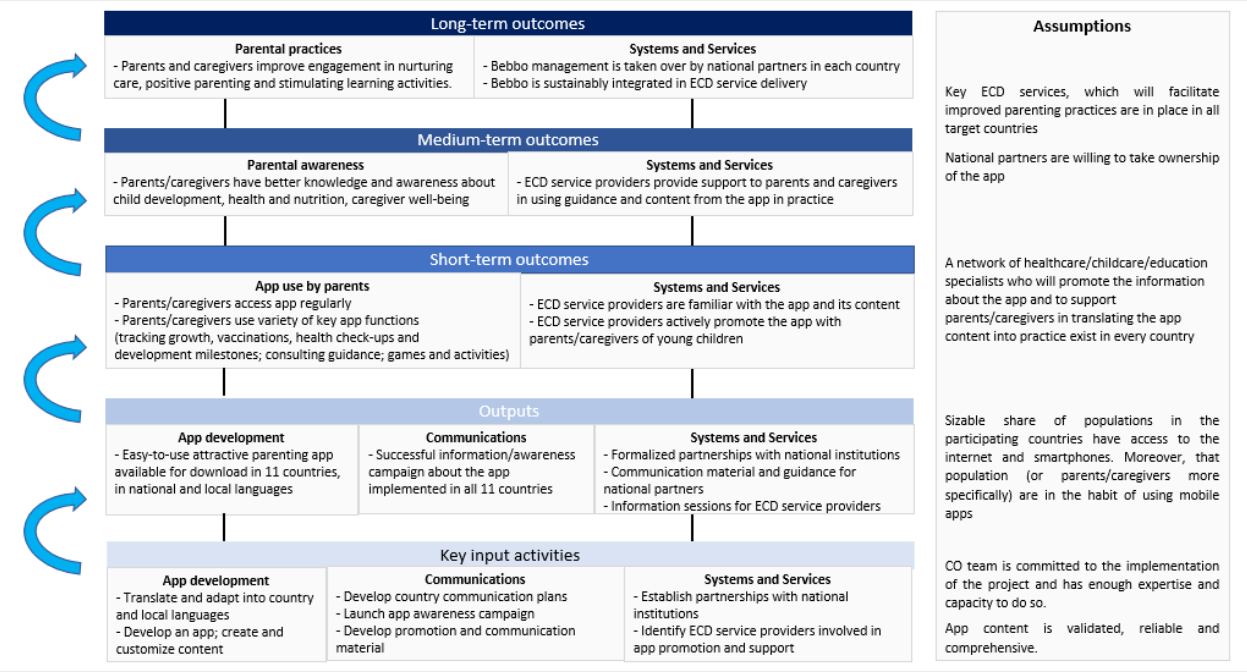
\includegraphics[width=\textwidth]{chapters/03-bebbo/images/bebbo-toc.png}
\caption{Bebbo Theory of Change}
\label{fig:Bebbo TOC}
\end{figure}


\section{Evaluation Questions and Methodology}

\subsection{Evaluation Questions}

Bebbo has benefited from regular monitoring exercises plus a few formative qualitative studies to improve its effectiveness. However, these are not enough to make a causal claim about the effects of Bebbo on children. Under this backdrop, the current evaluation is focused on the evaluation criteria of impact and has the overall objective of evaluating the causal impact of Bebbo with respect to the targeted outcomes of knowledge and awareness of key aspects of child development and parenting (medium-term outcomes) and parental engagement in nurturing care, positive parenting practices, engagement in stimulating and learning activities (long-term outcomes) for parents of 0-6 years old children.
Under a randomized encouragement design, described in the next section, the current multi-country experimental evaluation seeks to answer the following questions among a sample of Serbian and Bulgarian parents of 0-6 years old children:

\begin{enumerate}
\item Is promoting Bebbo an effective policy to improve parents’ knowledge and awareness about child development and health, as well as their parenting confidence and attitudes?
\item Is promoting Bebbo an effective policy to  improve positive parenting practices?
\end{enumerate}


\subsection{Measurement and key outcomes of interest}

Below we provide the description of measures used in the current study. Several measures for each construct have been piloted with an online survey prior to the main data collection (with a sample of approximately 200 parents) and analyzed for psychometric properties, having sufficient variance and no ceiling or floor effects. The following items/scales were kept for the main study. It should be noted that the survey was purposefully kept short to avoid high attrition rates as the recruitment of participants and longitudinal data collection was completely online.

\subsubsection*{Knowledge and awareness about child development and health}

To assess knowledge and awareness on child development, parents were asked how to monitor the development of their child with 4 items (items: “I know how to monitor the language development of my child”, “I know how to monitor the cognitive development of my child”, “I know how to monitor the social-emotional development of my child”, “I know how to monitor the physical development of my child”). The knowledge questions were further complemented with quiz-type true/false questions to measure parents’ knowledge of child developmental processes, adapted from the Knowledge of Infant Development Inventory (KIDI) and used in the Early Childhood Longitudinal Study, Birth Cohort (ECLS-B) study (example item: “Most 2-year-olds start to sort and pair things”).  However, these are excluded from analysis due to low reliability and unexpected behavior of the construct.

For health awareness and knowledge, parents were asked on whether they know about the vaccination related needs of their children with the following item: “I know which vaccine my child needs to take next”.

\subsubsection*{Confidence and attitudes}
Parents were asked how confident they feel in their ability to deal with their child’s emotions and how confident they feel in their ability to respond properly when their child misbehaves, on a 4-point Likert type scale (1=Not confident at all, 4=Very confident).
Attitude towards physical punishment was assessed with the following item from the UNICEF MICS Child Discipline module3: “Do you agree that in order to bring up, raise, or educate a child properly, the child needs to be physically punished?”, on a 4-point Likert scale (1=Do not agree at all, 4=Strongly agree).

\subsubsection*{Parenting practices}

Parental engagement was measured using the parental engagement subscale of the UNICEF MICS Early Childhood Development Index module. Participants were asked to report if they were engaged in six parental activities such as reading books, telling stories, singing songs, taking the child outside, playing with the child and naming, counting, and drawing with the child in the last 24 hours. The answer for each activity was coded as either 1 (yes) or 0 (no).
Positive affect and hostile parenting practices were measured using the two relevant subscales of the Preschool Parenting Measure. The positive affect subscale measures the warmth and affection involving parent-child interaction (4 items, example item: “I often smile when I am around my child”); and the hostility subscale measures harsh interactions between the parent and child (4 items, example item: “When my child does something wrong, I sometimes threaten her”, on a 4-point Likert scale (1=Do not agree at all, 4=Strongly agree).
Breastfeeding practices of parents of 0-2 years old children were measured with the following yes/no item: “Has your child been breastfed in the last 24 hours?”

In Table \ref{tbl:Reliability: Pooled Alpha Matrix}, we present the summary of number of items for the measures and also the reliability of scales used. Constructs with a reliability above 0.70 are considered internally consistent.

\input{chapters/03-bebbo/descriptives/tables/Reliability: Pooled Alpha Matrix}

\subsection{Sampling, recruitment, and data collection}

First, we conducted an initial pilot study in Bulgaria to assess the recruitment strategy's cost-effectiveness, along with the incentive amount and mechanism. As a result, we needed to deviate from the original plan due to budget and time constraints, leading to the inability to stratify as intended. Despite this deviation, the study remained powered to yield results, as later demonstrated.

Participants were recruited to the study with social media ads on the Meta platform (Facebook and Instagram) using the Virtual Lab platform to create and run the recruitment ads. The Virtual Lab platform is used to track and measure the price-per-respondent across multiple strata. It solves the core problem of monitoring, computing expectations, and adjusting budget when recruiting samples via social media platforms while ensuring they are representative across desired and measured characteristics.

In exchange for participating in the study, participants were told they could receive gift cards worth up to 12 USD (in their local currency). These gift cards were delivered as \$4 visa international gift cards in three rounds, which could be spent online but had to be spent for a purchase under \$4. See Figure \ref{fig:Recruitment Ads} for examples of the ad material used for recruiting.

\begin{figure}[H]
\centering
\begin{subfigure}{0.3\textwidth}
\centering

\includegraphics[width=100px]{chapters/03-bebbo/images/recruitment/558.png}
\end{subfigure}
\begin{subfigure}{0.3\textwidth}
\centering
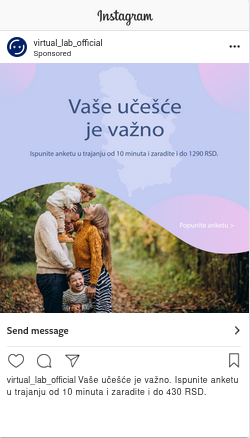
\includegraphics[width=100px]{chapters/03-bebbo/images/recruitment/639.png}
\end{subfigure}
\begin{subfigure}{0.3\textwidth}
\centering

\includegraphics[width=100px]{chapters/03-bebbo/images/recruitment/742.png}
\end{subfigure}
\caption{Recruitment Ads}
\label{fig:Recruitment Ads}
\end{figure}

The survey was administered via a chatbot in Facebook Messenger, using the Virtual Lab platform. Respondents who clicked on the advertisements were directed to a Messenger chat with the Virtual Lab Facebook page, which did not contain any content or information related to this study. Consent was provided via chat, as well as all answers to the survey questions and the treatment condition. Gift cards were also provided via chat, using the Tremendous gift card platform to provide Visa international prepaid cards. The Virtual Lab chatbot allowed the researchers to create multi-wave surveys, with independent timing. It additionally allowed the easy provision of gift cards at the end of each wave, which is integrated into the survey directly via the platform.

Ads were broadly targeted to all Meta users between the ages of 20-40. The inclusion criteria for sampling was to have a child between 0-6 years old. In case of having more than one 0-6 years old child, parent/main caregiver was asked to select one focal child and respond to the questions considering that focal child.

The data collection was longitudinal in which we measured the outcomes of interest before treatment (in a baseline survey) and after treatment (in an endline survey). We added an additional survey after the endline, referred to as a follow up, to look for longer-term impacts concerning the behaviors and test the impact of continued app usage. Recruitment and survey administration was performed on a rolling basis between March and October, 2023. Each individual participant was treated at the end of the baseline survey and sent the endline survey 4 weeks after completing the baseline survey.


% \vspace{1cm}
\begin{figure}[H]
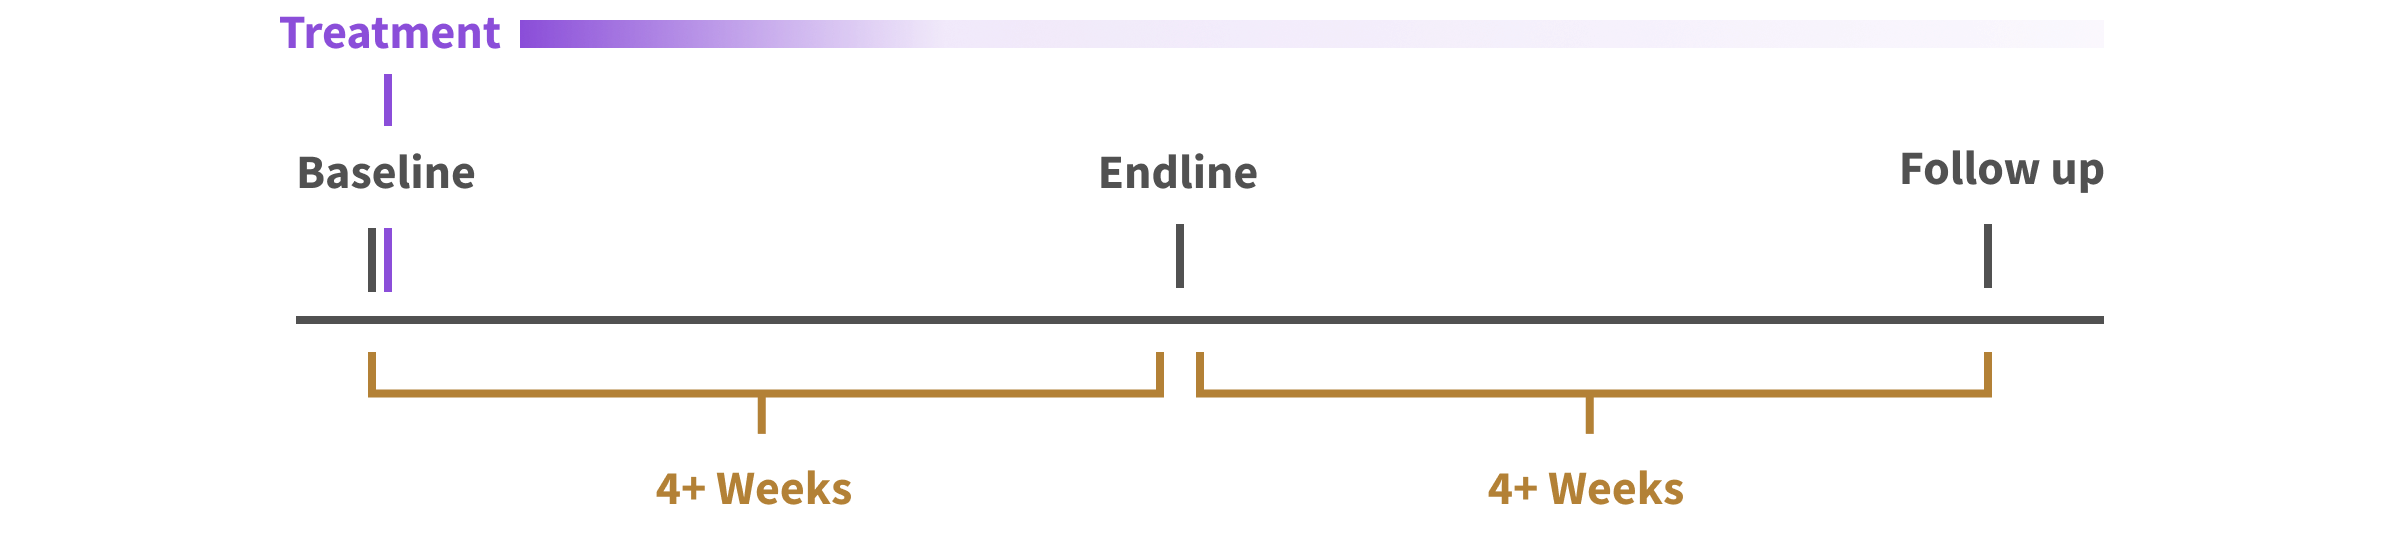
\includegraphics[width=\textwidth]{chapters/03-bebbo/images/design-timeline.png}
\caption{Study Design}
\label{fig:Study Design}
\end{figure}

\subsection{Experimental Design}

This study follows a prepost design (\cite{Clifford2021}) in which we measure the outcomes of interest before treatment (in a baseline survey) and after treatment (in an endline survey). We add an additional survey after the endline, referred to as a follow up, to look for longer-term impacts and test the impact of continued app usage. To answer the evaluation questions, a randomized controlled encouragement design is conducted, in which study participants are randomized to one of the two following conditions upon taking the baseline survey:

\paragraph{Treatment.} Participants in the treatment condition were told that there was one more step to qualify for the study and were then asked to download the app Bebbo and use it regularly, being encouraged that doing so will help them with their parenting.

\paragraph{Control.} Participants in the control condition were told that there was one more step to qualify for the study and were then provided a link to a basic website containing information on parenting and asked to visit it regularly, being encouraged that doing so will help them with their parenting.

This evaluation, which benefits from a randomized encouragement design where potential users are invited (i.e., encouraged) to use Bebbo, was necessitated by the self-administered nature of Bebbo as a mobile app-based intervention. This also follows Moayyedi and Hunt \parencite*{Moayyedi2014}, which advise the use of encouragement designs in situations where a solution is widely available and people cannot be forced to use it.  It is also in line with one way in which Bebbo has been implemented in real life, through promoting the app on the web (e.g., in social media platforms) and other platforms and expect users to download the app and use it at their own discretion.

We consider “an effective policy” one which performs better than the “treatment as usual” case, which we will consider to be an existing, static website. Finally, we are studying the general population of caregivers of young children. No particular care was given to single out any particular subset of the population that might benefit the most (or the least) from Bebbo, nor those who would be most likely to use Bebbo.




\subsubsection*{Treatment Condition}
Participants were sent the following message at the end of the baseline survey:

\begin{quote}
There is just one more step to qualify for the Visa gift card of X. Please download Bebbo, the free parenting app, and discover how it can help you. Using Bebbo regularly can improve your interactions with your children and help you support their development better! You can do so by clicking the link below:
\end{quote}

Clicking on the link led them to the Bebbo app page where they were invited to download the app via the app stores (Google or Apple). App usage in the treatment group was tracked via tracking ids sent with the link to the app download page, allowing us to follow the app usage of each individual treatment participant and measure take-up. If someone decided to ignore the page, and instead went on their own to search for and download Bebbo, we would not have data on their usage. Thus, usage data and take-up should be considered a lower bound. Additionally, if someone had previously downloaded the app, we would not have information about their usage in this period, but those participants would be considered always takers” and the lack of information about their usage does not impact the effect.

The Bebbo app is designed so that parents can begin using the app by creating a ”profile” of their child, entering basic information such as when she was born. After this, the parent is shown relevant content, asked to track milestones, and offered suggestions for content reading or games to play with their child.

We collected all app usage events. For the sake of our study, we were interested in a subset of events that represented the accessing of content or features that contained information or might impact their behavior. A set of six events were determined to fit the bill, namely: advise details opened, game details opened, child milestone tracked, child measurement entered, child vaccine entered, and child health checkup entered.

\subsubsection*{Control Condition}
Participants were sent the following message at the end of the baseline survey:

\begin{quote}
There is just one more step to qualify for the Visa gift card of X. Please visit the following free parenting website and discover how it can help you. Using this website regularly your interactions with your children and help you support their development better! You can do so by clicking the link below:
\end{quote}

The choice to use a website as a treatment-as-usual (TAU) condition was decided by the evaluation and program team because it represented an alternative (and traditional/existing) way to solve the problem that the Bebbo app was trying to solve. Another option that was considered was to use an alternate parenting app, but the team believed that using a website gave the best chance to detect a difference in the use of an app, rather than the specific implementation of the Bebbo app.

The most “basic” website was selected as treatment as usual (TAU). The website was chosen so as to be “static” (showing the same content to everyone rather than allowing user to create individualized profiles) so that it acted as an informational resource rather than a web app or platform which would similarly overlap with the concepts behind the Bebbo app.

The downside with choosing a treatment-as-usual condition is that if one does not find significant effects of the treatment, one cannot differentiate between the following scenarios:

\begin{enumerate}
\item The control is effective and the treatment equally effective.
\item Neither the control nor the treatment are effective.
\end{enumerate}

The assumption with this impact evaluation, from a policy perspective, is that the two are equally important. If the development and promotion of a new app does not improve parenting knowledge beyond what already exists in the market, then it is not an effective investment for public funds. That being said, there is some evidence in this study that allows us to differentiate between the two scenarios and determine that it is likely the latter. In particular, we conclude that neither control nor treatment condition make any significant impact on the general population above and beyond the priming effect of the baseline survey itself (to be discussed in depth in the section with results).

\subsection{Power Analysis}

The total number of participants to be recruited into the study at baseline is determined to be 1500 per country, following an a priori statistical power analysis assuming a power of 80\%, significance level of 5\% (two-tailed), medium effect size of Cohen’s d=0.5, and adjusted for anticipated rates of 30\% take-up, and 30\% baseline-to-posttest and 15\% posttest-to-follow up attrition.

Furthermore, ex-post power analysis is provided to show the ability to detect an effect, in terms of standardized deviations (corresponding to Cohen’s d effect sizes), in the datasets analyzed. To create the effect size, the standardized difference is multiplied by the empirical take-up of 30\%, which was the percentage of participants that had at least one learning event in the treatment group. The results show that the study is well powered (above 80\%) to detect a medium effect size (0.5 standard deviations) on the difference between endline and baseline surveys, even when that effect is entirely limited to the 30\% take-up group, at a significance level of 5\%. We also provide plots showing the power at 1.25\%, to show the equivalent of a 10\% significance level after controlling for multiple testing (8 outcomes) with a Bonferroni correction. See Appendix Figure \ref{fig:Power Analysis}. Thus, the study is well-powered to determine whether or not the 30\% who used the app were impacted.


\section{Preliminary Analysis}

\subsection{Respondent characteristics by country}

Table \ref{tbl:Baseline Respondent Characteristics} provides the baseline characteristics of the respondent population, separated by country. Note that these are also the control variables we use in all regressions.

Most respondents were themselves parents (not grandparents or other caregivers), women, under 35 years of age, and spoke the dominant language of the country at home. A little over half had children 2-6, compared to 0-2 years of age. Respondents in Bulgaria were more likely to have a university education (42\%) compared to those in Serbia (29\%), but in both cases the majority of respondents did not have a university education

\input{chapters/03-bebbo/descriptives/tables/Baseline Respondent Characteristics}

\subsection{Descriptive statistics}

Descriptive statistics regarding the baseline responses for the outcomes are shown in Table \ref{tbl:Outcome Construct Descriptives Pooled Baseline}. Note that many of the constructs have quite high means and medians and some have a high proportion of respondents with the max score. In particular, 74\% and 75\% of respondents scored perfectly on the knowledge questions (where vaccine knowledge was only asked to those with a child aged 0-2). This is problematic, as knowledge is often considered the easiest to change quickly and was a core outcome of interest for the team. Additionally, knowledge questions seem to be heavily impacted by the repeated survey effect, as discussed further down.

\input{chapters/03-bebbo/descriptives/tables/Outcome Construct Descriptives Pooled Baseline}

\subsection{Prexposure to Bebbo}

This study recruited Serbian and Bulgarian caregivers online, via social media ads, and invited half of them to download the app Bebbo. What if some people were already familiar with the app? Or had already downloaded and used it before? This would not impact the internal validity of the study, however, it has implications for the external validity.

If someone had already downloaded the app and still had it on their phone, we would not be able to track their usage and they would be considered “non-compliant” in this design. This is desirable from an analysis perspective, as these people are “always-takers” (\cite{Imbens2015}) who would have the app regardless of whether they were assigned the treatment or control condition.

To check for such “pre-exposure,” we ask control group users, at the end of the final follow up survey, if they have ever heard of or used Bebbo.

55\% of respondents said that they had heard about the app Bebbo and 23\% said that they had downloaded and used the app Bebbo. It’s worth noting that there might be some social desirability bias or acquiescence bias (\cite{Stantcheva2023}) in these responses and we do not have a good way to detect that in this instance. However, despite those potential biases, this is strong suggestive evidence that there was pre-exposure to the treatment in our sample. This has no internal validity implications but does bound the interpretability of the results. Assuming high usage among respondents that claim to use the app, we would then say this is the impact of engaging new users in a country already familiar with Bebbo.

\subsection{Attrition and survey behavior}

\subsubsection*{Attrition}

About 52\% of those who started the survey dropped off before completing it and 54\% never came back from the baseline to complete the endline. Attrition between endline and follow-up was 66\%. Table 4 summarizes attrition by stage and treatment condition. It’s worth noting that attrition was consistently higher among the treatment group, possibly related to the increased number of questions in the endline survey for that group (additional questions about app usage were added for the treated).\footnote{An error in survey coding led to a portion of early respondents receiving “switched” end-line surveys. This potentially contaminated the control group. To ensure the robustness of the analysis, the contaminated sample was discarded from the follow-up survey analysis.}

The attrition rates follow those of online surveys which range from 30\% to 50\% (\cite{zhou2016pitfall}). This becomes an issue of validity only if attrition rates are different between treatment and control groups. To test for this, we conduct a selective attrition test (\cite{ghanem2023testing}). Table \ref{tbl:Attrition: Pooled} shows that attrition occurred at the same rate between control and treatment groups and as such it is not a threat for internal validity.

\input{chapters/03-bebbo/descriptives/tables/Attrition: Pooled.tex}

\input{chapters/03-bebbo/regressions/Attrition Prediction (All).tex}

\subsubsection*{Follow-up time}
Note that respondents should have been contacted 4 weeks after each wave in order to take the subsequent wave. However, two factors may have led to them not always starting the wave after exactly 4 weeks: (i) there were some technical issues which caused the notification to be delayed in some cases and (ii) not everyone begins the survey immediately when notified and maybe need to be reminded several times, or may remember on their own, significantly later.

To improve consistency of the study, we removed anyone who took the endline or follow-up surveys more than 9 weeks after their previous survey, ensuring that all respondents were responding in a gap between 4-9 weeks. Table \ref{tbl:Time Gap Descriptives} summarizes the distribution of this time gap. As you can see, the vast majority (more than 80\%) took the survey after 4-5 weeks of the previous survey.

\input{chapters/03-bebbo/descriptives/tables/Time Gap Descriptives}

\subsection{Baseline balance}


To test for balance between our randomly assigned treatment and control groups, we run an omnibus test, following Hansen and Bowers \parencite*{Hansen2008}, to observe standardized differences at baseline and the associated omnibus p-value. Results are reported separately for each country and found in Table \ref{tbl:Baseline Balance Serbia} and Table \ref{tbl:Baseline Balance Bulgaria}. Following Altman \parencite*{Altman2014}, we do not change our analysis plan based on these results, but it is worth noting that the Bulgaria data does seem to suffer from slight unusual differences between treatment and control condition and the p-value of the omnibus test is low. All the analysis is also reported for only those respondents in Serbia as well, which serves as a robustness check against any concerns that Bulgarians were randomized into unlucky groups for our analysis.

\input{chapters/03-bebbo/balance/Baseline Balance Serbia}
\input{chapters/03-bebbo/balance/Baseline Balance Bulgaria}

\subsection*{App Usage Characteristics}


To measure takeup, we pick how many distinct days the participant used the app, as measured by one of the predefined set of ``learning events'' that include looking at material or entering milestones for their child. Note that in order to generate a ``learning event,'' one must get past the ``welcome'' screens and create a profile for their child.

Figure \ref{fig:treatment-takeup-histogram} and Table \ref{tbl:Treatment Takeup} shows some take-up numbers for different intensities of usage. Very few treated respondents used the app more than three days (less than 3\%) and only about 12\% used it more than once. The maximum group of 8 people, less than 1\% of the population treated, used the app on more than 5 days in the 4-6 week period. The usage characteristics of the 305 users who did use the app is visualized in a histogram in Figure 3, which shows how many days they used the day.

Additionally, Table \ref{tbl:App Engagement (30 days)} shows app engagement for those that did download the app, including data from app usage in Serbia and Bulgaria that was not associated with the study. Note that, of those who did download the app in the study (and therefore were complying with the recommendations of the study) only about 55\% actually finished creating a profile for their child and only 24\% used the app past the first day and 5\% used it for more than 3 days.

For additional context, we provide table \ref{tbl:App Retention Funnel (Non Study)} to show a full retention funnel for all users who downloaded in the first eight months of 2023 outside of our study. The numbers are worse for those outside of the study. Note that the engagement numbers in were restricted to 30 days after downloading, to compare with the timeframe between baseline and endline within the study. This comparison to outside-study users is important, as it emphasizes the external validity of these findings. Users outside the study used the app less intensively than those in the study implying an upward bias on effect sizes of any impact within this study.

Altogether, these findings indicate that the app is not engaging for the majority of caregivers who agree to download it. The Theory of Change for Bebbo relies on caregivers using the app regularly and their engagement with its different components. At the moment, Bebbo has retention rate issues, with the most important issues being on initial download


\begin{figure}[H]
  \centering
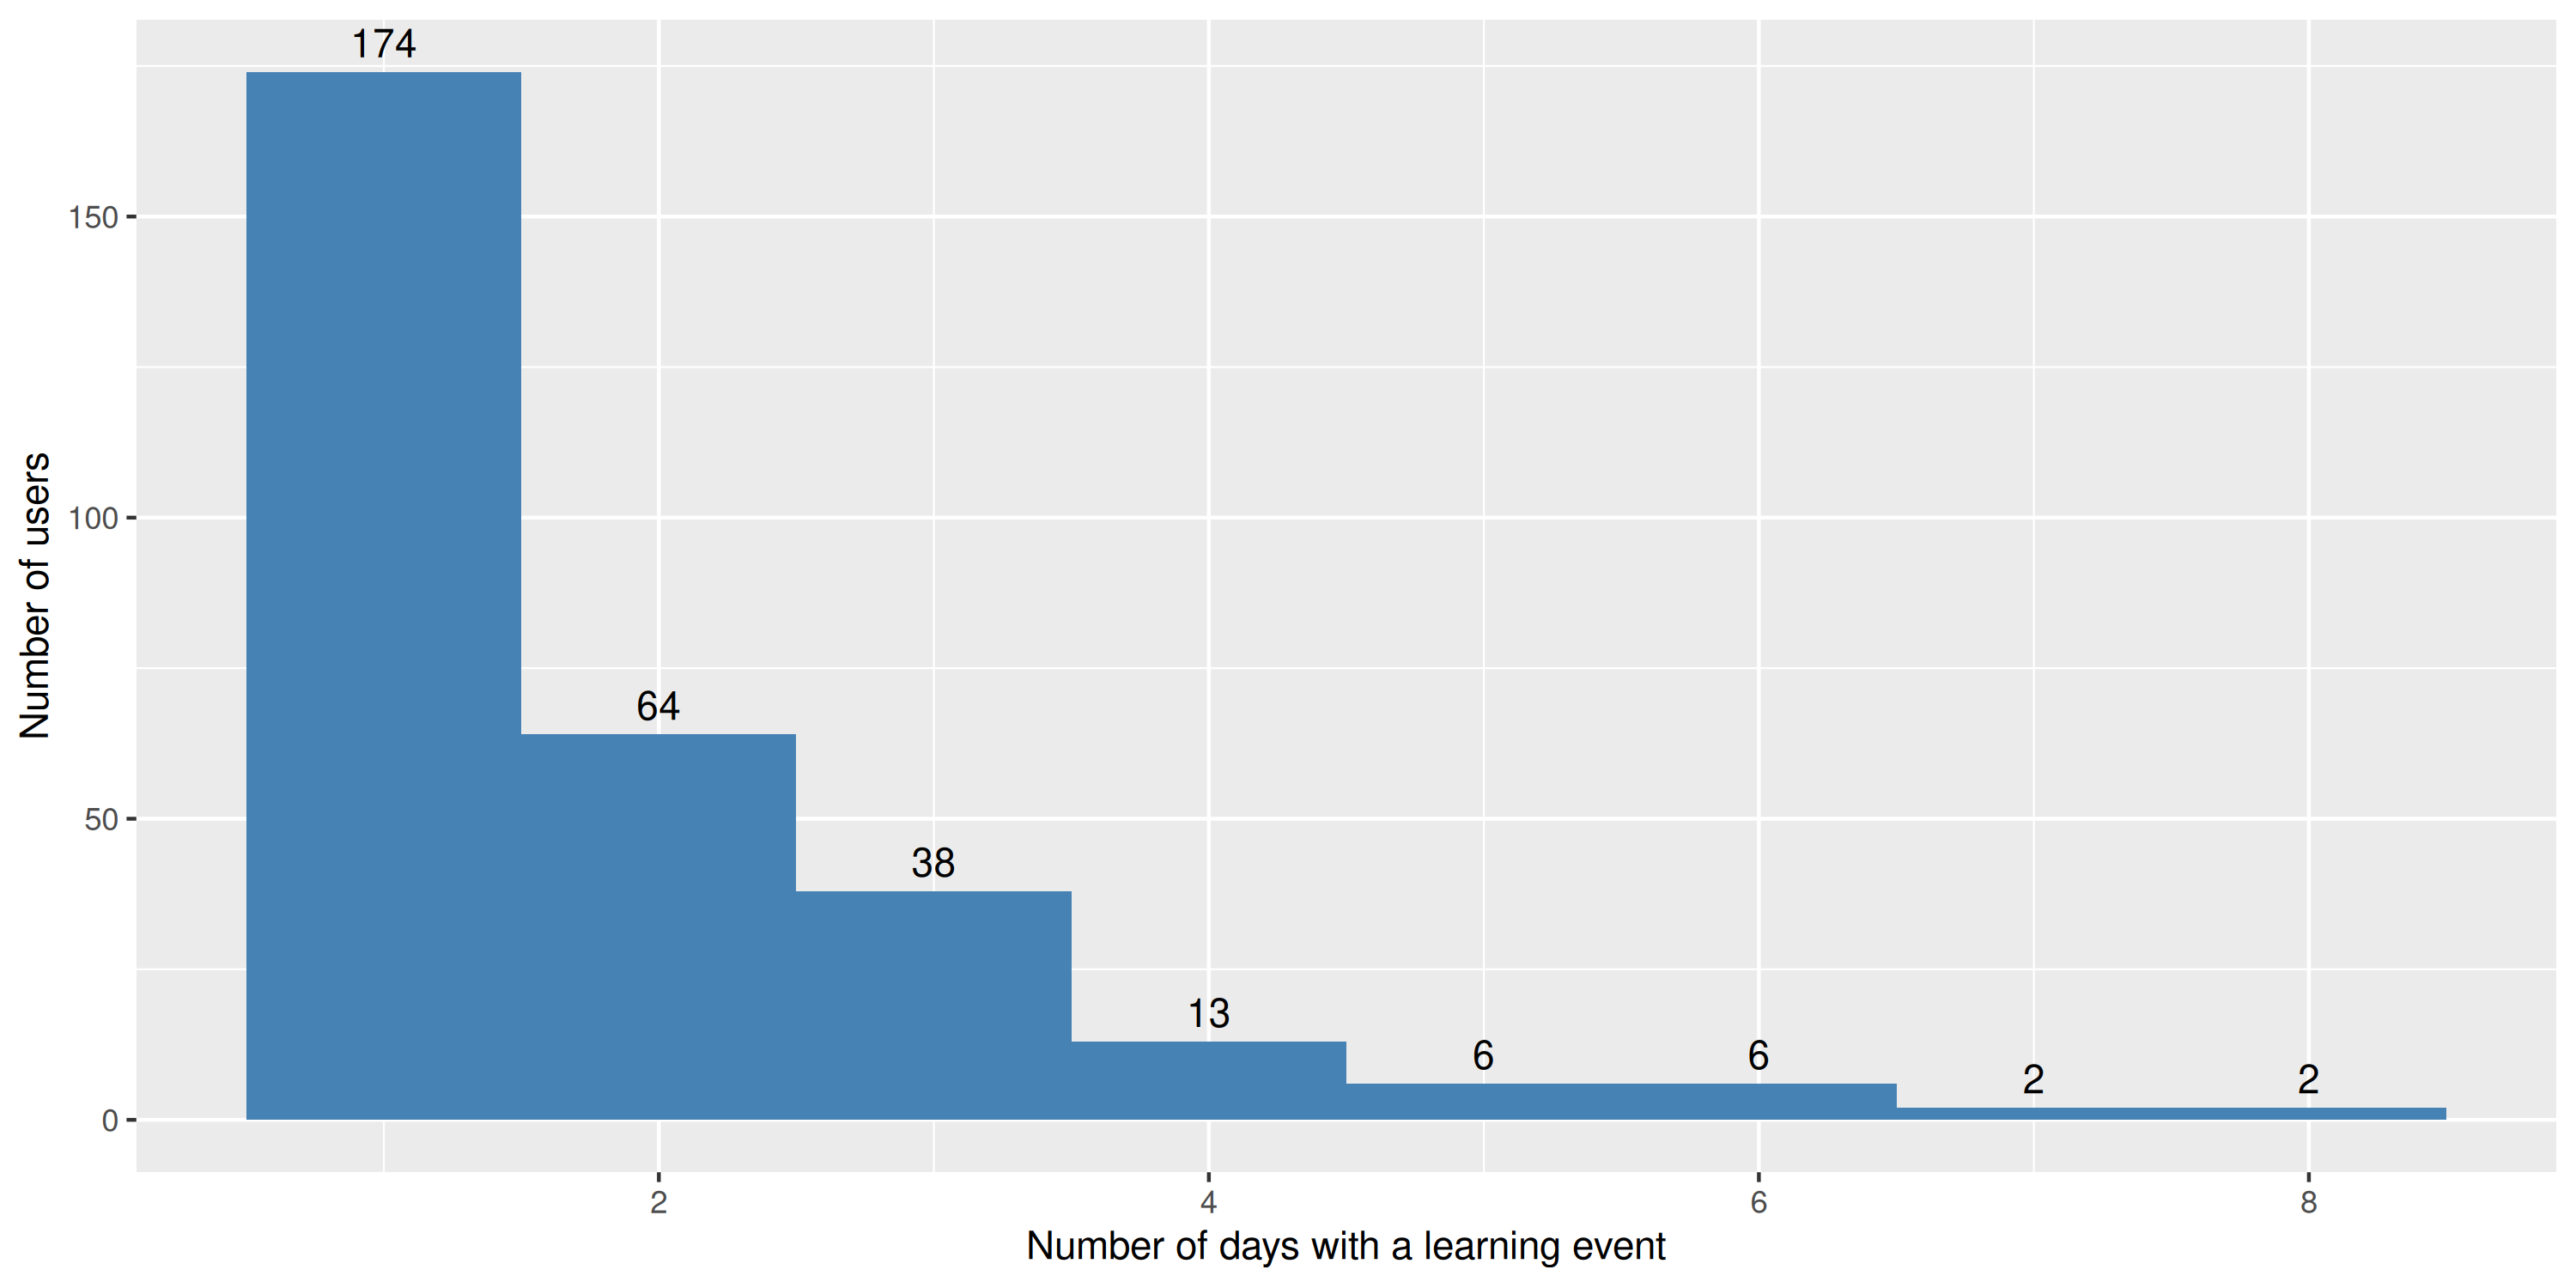
\includegraphics[width=\textwidth]{chapters/03-bebbo/plots/Treatment Takeup Baseline - Endline.png}
\caption{Days with Learning Event (Baseline - Endline)}
\label{fig:treatment-takeup-histogram}
\end{figure}


\input{chapters/03-bebbo/descriptives/tables/Treatment Takeup}

\input{chapters/03-bebbo/descriptives/tables/App Engagement (30 days)}

\subsection{Long Term User Retention}

For additional context, we use the Bebbo app analytics database (Firebase data stored BigQuery) and create a user-retention funnel which gives us information about longer-term app usage in a real-world context outside of this study.

We pull data for users who have a “first app open” event between January 1, 2023 (inclusive) and October 1, 2023 (exclusive). We then restrict our analysis to events within 6 months of their first app open event to create a uniform window for analysis. We measure how many people who downloaded (opened) the app ended up setting up a profile and accessing learning content (“used”) and track how many access learning content after the first day, after 30 days, after 60 days, and after 90 days.

This data is provided in Table {\ref{tbl:App Retention Funnel (Non Study)}}. These numbers show that less than 30\% of downloaders actually complete a profile and access content. Then, only 20\% of downloaders returned to the app after the first day, with 16\% remaining after 30 days.

The similarity to the 30-day non-study usage emphasizes that users who do not use the app within the first 30 days of downloading will generally not use the app at all in the first 6 months and potentially ever.

\input{chapters/03-bebbo/descriptives/tables/App Retention Funnel (Non Study)}


\subsection{User characteristics correlated with app usage}

Given that so few caregivers used the app, it seems important to ask the question: “who are the respondents who end up as app users?” We do so by regressing respondents’ app usage activity between baseline and endline against their characteristics at baseline. In particular, we will pick three binary outcomes: those who had at least one learning event, who we will say “Used the App,” those who had learning events on at least two days, or “Used More Than 1 Day,” and finally, those who used the app more than three days.

The results can be found in Table \ref{tbl:App Usage (All)}. The regression is formulated as a simple linear regression for ease of interpretability. The most notable predictor is whether or not the participant is the parent of the child. The other notable predictor is “Activities Past 24h” which is aligned with what we see in the raw data (under Results). It does seem that in our sample, those who reported doing fewer activities together with their child are more likely to download and use the app.

One possible interpretation could be that there is a set of people who are not likely to spend time with their children but are likely to download and use apps. Unfortunately, we do not see a positive impact of this app on those people spending more time with their children, but potentially on a narrow subgroup there might be a positive impact that we do not detect. This could indicate that for “screen parents” that are not currently spending time with their children, an app is an effective way to get in front of them. The open question is whether or not it improves their behavior.

There is some additional evidence that those with young children are more likely to use the app, along with those who have less knowledge of child development, speak the dominant language, and are university educated. However, preliminary analysis shows no impact among this group (see appendix tables \ref{tbl:Only Children 0-2: OLS - Endline - Knowledge and Awareness}-\ref{tbl:Only Children 0-2: OLS - Endline - Practices}).

\input{chapters/03-bebbo/regressions/App Usage (All)}

\input{chapters/03-bebbo/regressions/App Usage (With Children 0-2)}


\section{Findings}

We run the following regression model to measure the intent-to-treat effect (ITT) of assignment to the treatment arm:
$$
y_{i} - y^{b}_i = \gamma_1 + \beta T_{i} + \gamma_2X_{i} + \epsilon_i
$$

Where $y_i$ represents the outcome of interest for individual $i$ measured after treatment, $T_i$ represents the random treatment assignment, $X_i$ a set of control variables and $y^b_i$ represents the outcome of interest measured before treatment. The parameter of interest will be the treatment effect, $\beta$.

Note that due to the relatively large number of sepearate outcomes (8), we adjust p-values of the treatment variable to control the false discovery rate (FDR), using Benjamini-Hochberg, reported as the ``Adjusted Treatment p-value.''

We also run the regression for two separate time periods: endline and follow-up. However, due to large attrition in the follow-up survey and the low long-term app takeup, the decision was made to rescope this evaluation to focus on the endline. Additional tables are available in the appendix.

One of the dangers of a prepost design is that you are priming your respondents with the first survey and that priming may impact how they answer the questions in the post-treatment survey(s) (\cite{Stantcheva2023}). Given this particular study design, where our control is a ``treatment as usual'' (TAU) that involved sharing a website and we do not have data regarding the takeup, or usage, of the website, it is difficult to isolate a priming effect.

We plot raw charts showing mean scores at baseline and endline for three groups for each variable: control, treatment with take-up (those who we know downloaded and used the app), and treatment without take-up (those for whom we have no data showing they downloaded or used the app). These plots can provide suggestive evidence of priming effects by showing the shift in mean between baseline and endline across all three groups. It’s worth noting that we cannot separate a priming effect from the effect of time itself, as it would be expected for parents to gain knowledge as time progresses.

Table \ref{tbl:Baseline Respondent Characteristics}, with the baseline respondent characteristics, shows all the control variables used. Note that several outcomes only applied to parents with children in a certain age group: ”Breastfed” and ”Vaccine Knowledge” applied to those with children ages 0-2. Thus, the binary control variable representing the age of the child (0-2 or 2-6) was removed in those regressions.

Finally, appendix tables \ref{tbl:Pooled: 2SLS - Endline - Knowledge and Awareness}-\ref{tbl:Pooled: 2SLS - Endline - Practices} show the results for the treatment effect on the treated (TOT) estimators. These are also not significant.


\subsection{Knowledge and Awareness}

Regression analysis of these outcome constructs show no significant result of treatment (Table \ref{tbl:Pooled: OLS - Endline - Knowledge and Awareness}).

\input{chapters/03-bebbo/regressions/Pooled: OLS - Endline - Knowledge and Awareness.tex}

These two constructs, Vaccine Knowledge and Child Development Knowledge, both suffered from ceiling effects in the baseline survey (72\% and 73\% respectively). On top of those ceiling effects, they both potentially suffered from priming effects, as evidenced by the consistent improvement in the endline survey for all groups.

Note that there is some evidence that those with less vaccine knowledge were more likely to download the app, indicating that takeup might be biased towards those who need it the most. This can be seen in the pre-post plots (Figure \ref{fig:knowledge-pre-post}) but it can be more formally seen in the regressions in the section App Usage, where the regressions with parents of children 0-2 also show evidence that vaccine knowledge is a predicter of continued app usage, in the inverse (those with less knowledge to begin with are more likely to keep using the app).

Unfortunately, we do not see this same impact on this subset of people even if we perform a subgroup analysis regression, which can be seen in the appendix in Appendix Table \ref{tbl:Vaccine Failures Subgroup OLS - Endline}. This indicates that while the app is more likely to be used by that group of people, it would seem that the control subgroup also improved their vaccine knowledge significantly thus canceling out any impact from the app usage.

These two constructs, Vaccine Knowledge and Child Development Knowledge, both suffered from ceiling effects in the baseline survey (72\% and 73\% respectively). On top of those ceiling effets, they both potentially suffered from priming effects, as evidenced by the consistent improvement in the endline survey for all groups.


\begin{figure}[H]
  \centering
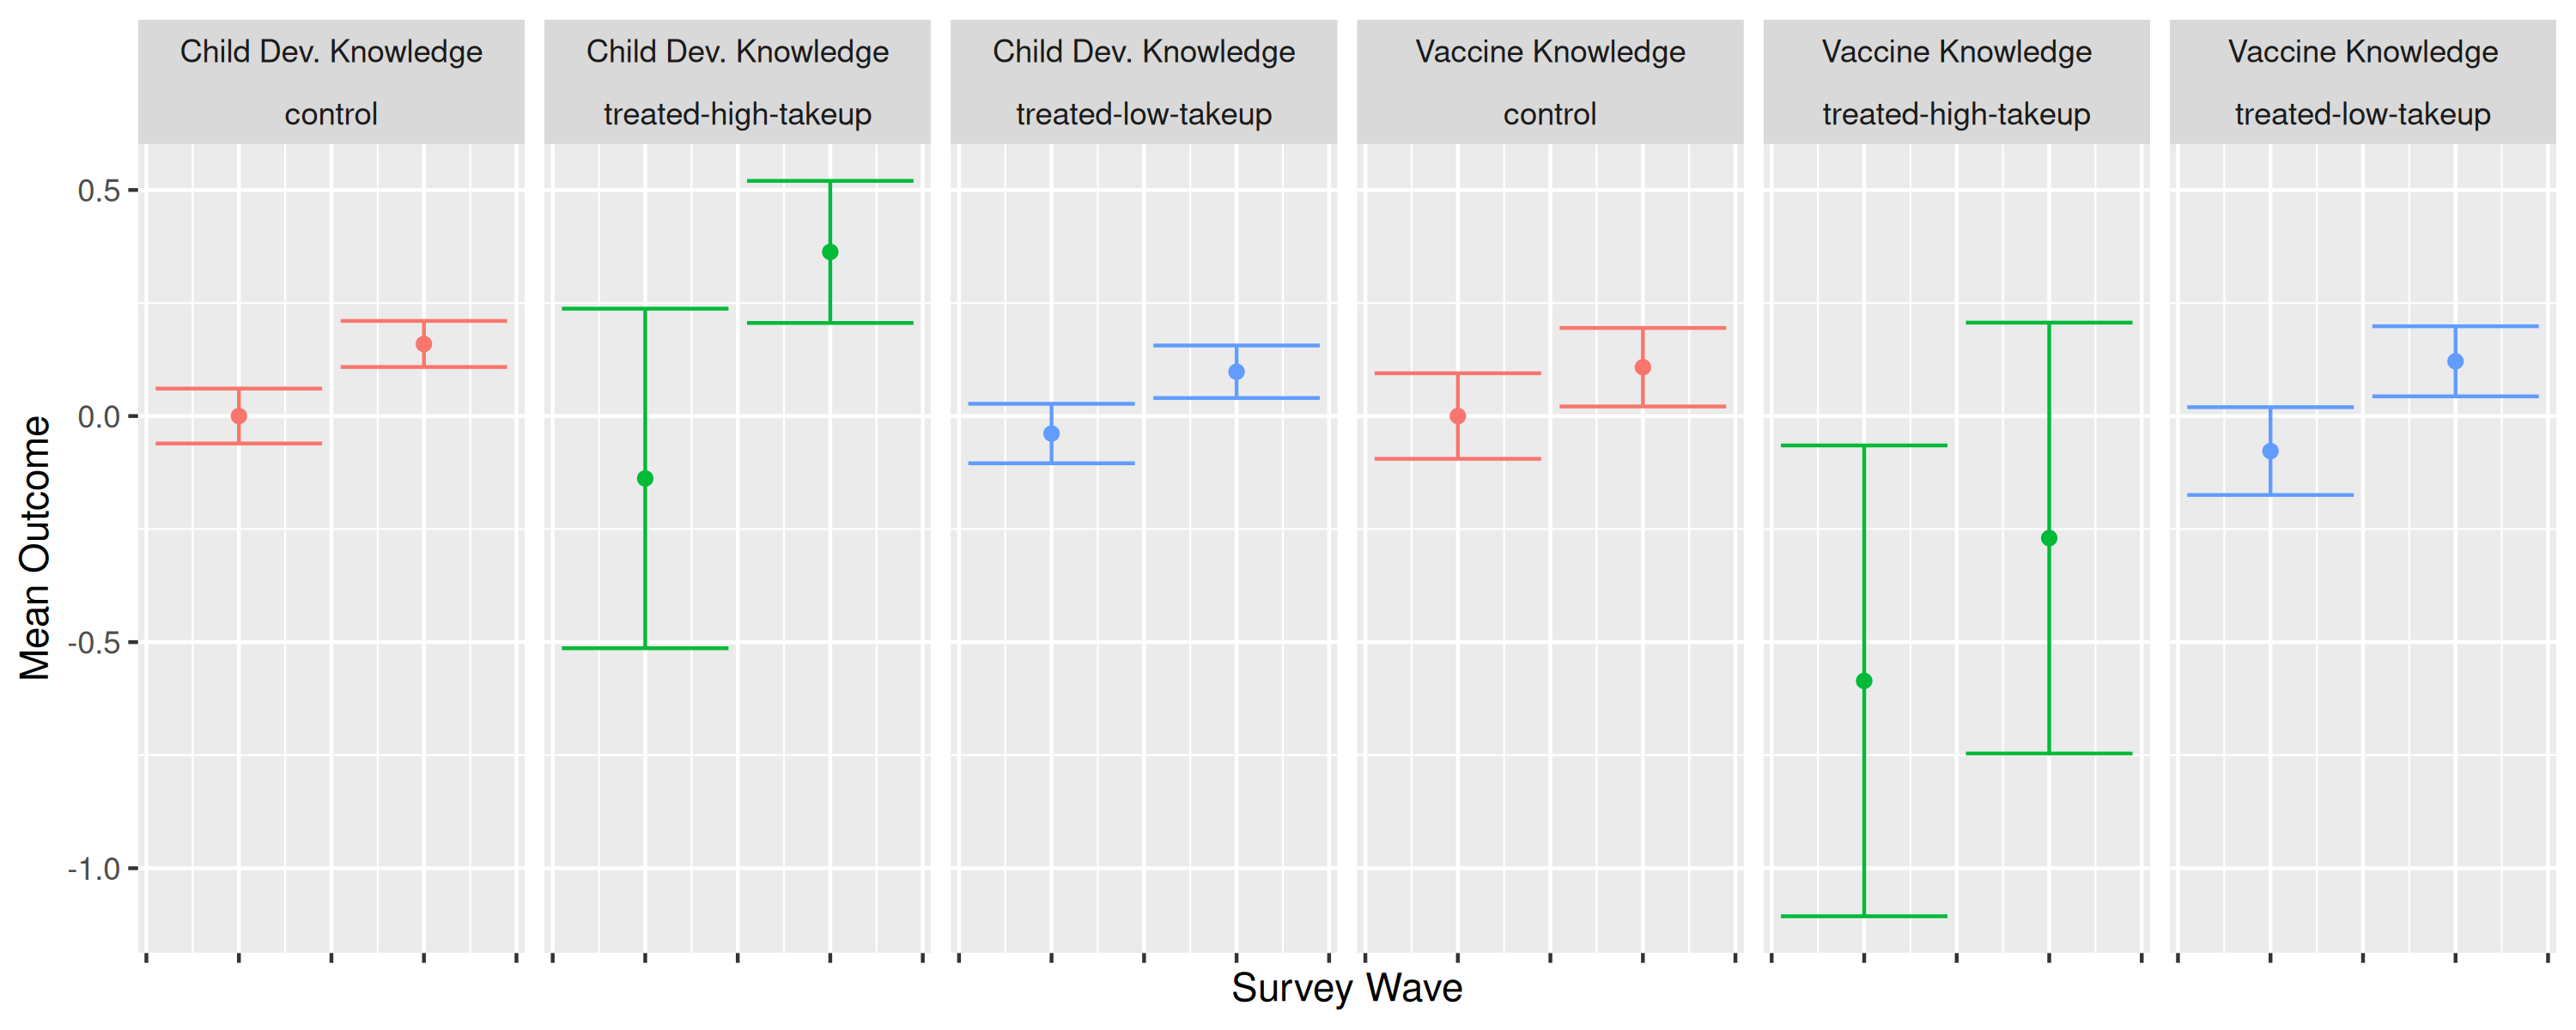
\includegraphics[width=\textwidth]{chapters/03-bebbo/plots/pre_post/Pooled: Vaccine Knowledge.png}
\caption{Knowledge and Awareness}
\label{fig:knowledge-pre-post}
\end{figure}


\subsection{Confidence and Attitudes}

Attitude Towards Physical punishment is a single question which asks if the parent believes the child needs to be physically punished. While there might seem to be some suggestive evidence from the coefficients of the regression model, the raw data shows that the positive coefficient is indicative of the fact that the control group got worse over time. They were more supportive of physical punishment in the endline survey. While there might be a story to that, it could also be the exact kind of statistical anomaly that multiple testing correction is designed to help us avoid when checking so many outcomes.

Parenting Confidence shows no significant impact in the regression analysis. The raw data shows suggestive evidence that those with lower confidence might be more likely to take up the treatment. The lack of a positive coefficient in the regression, however, might indicate that those in the control group were equally likely to take up either the control website or seek out information on their own in order to improve by endline.

\input{chapters/03-bebbo/regressions/Pooled: OLS - Endline - Confidence and Attitudes.tex}
\begin{figure}[H]
  \centering
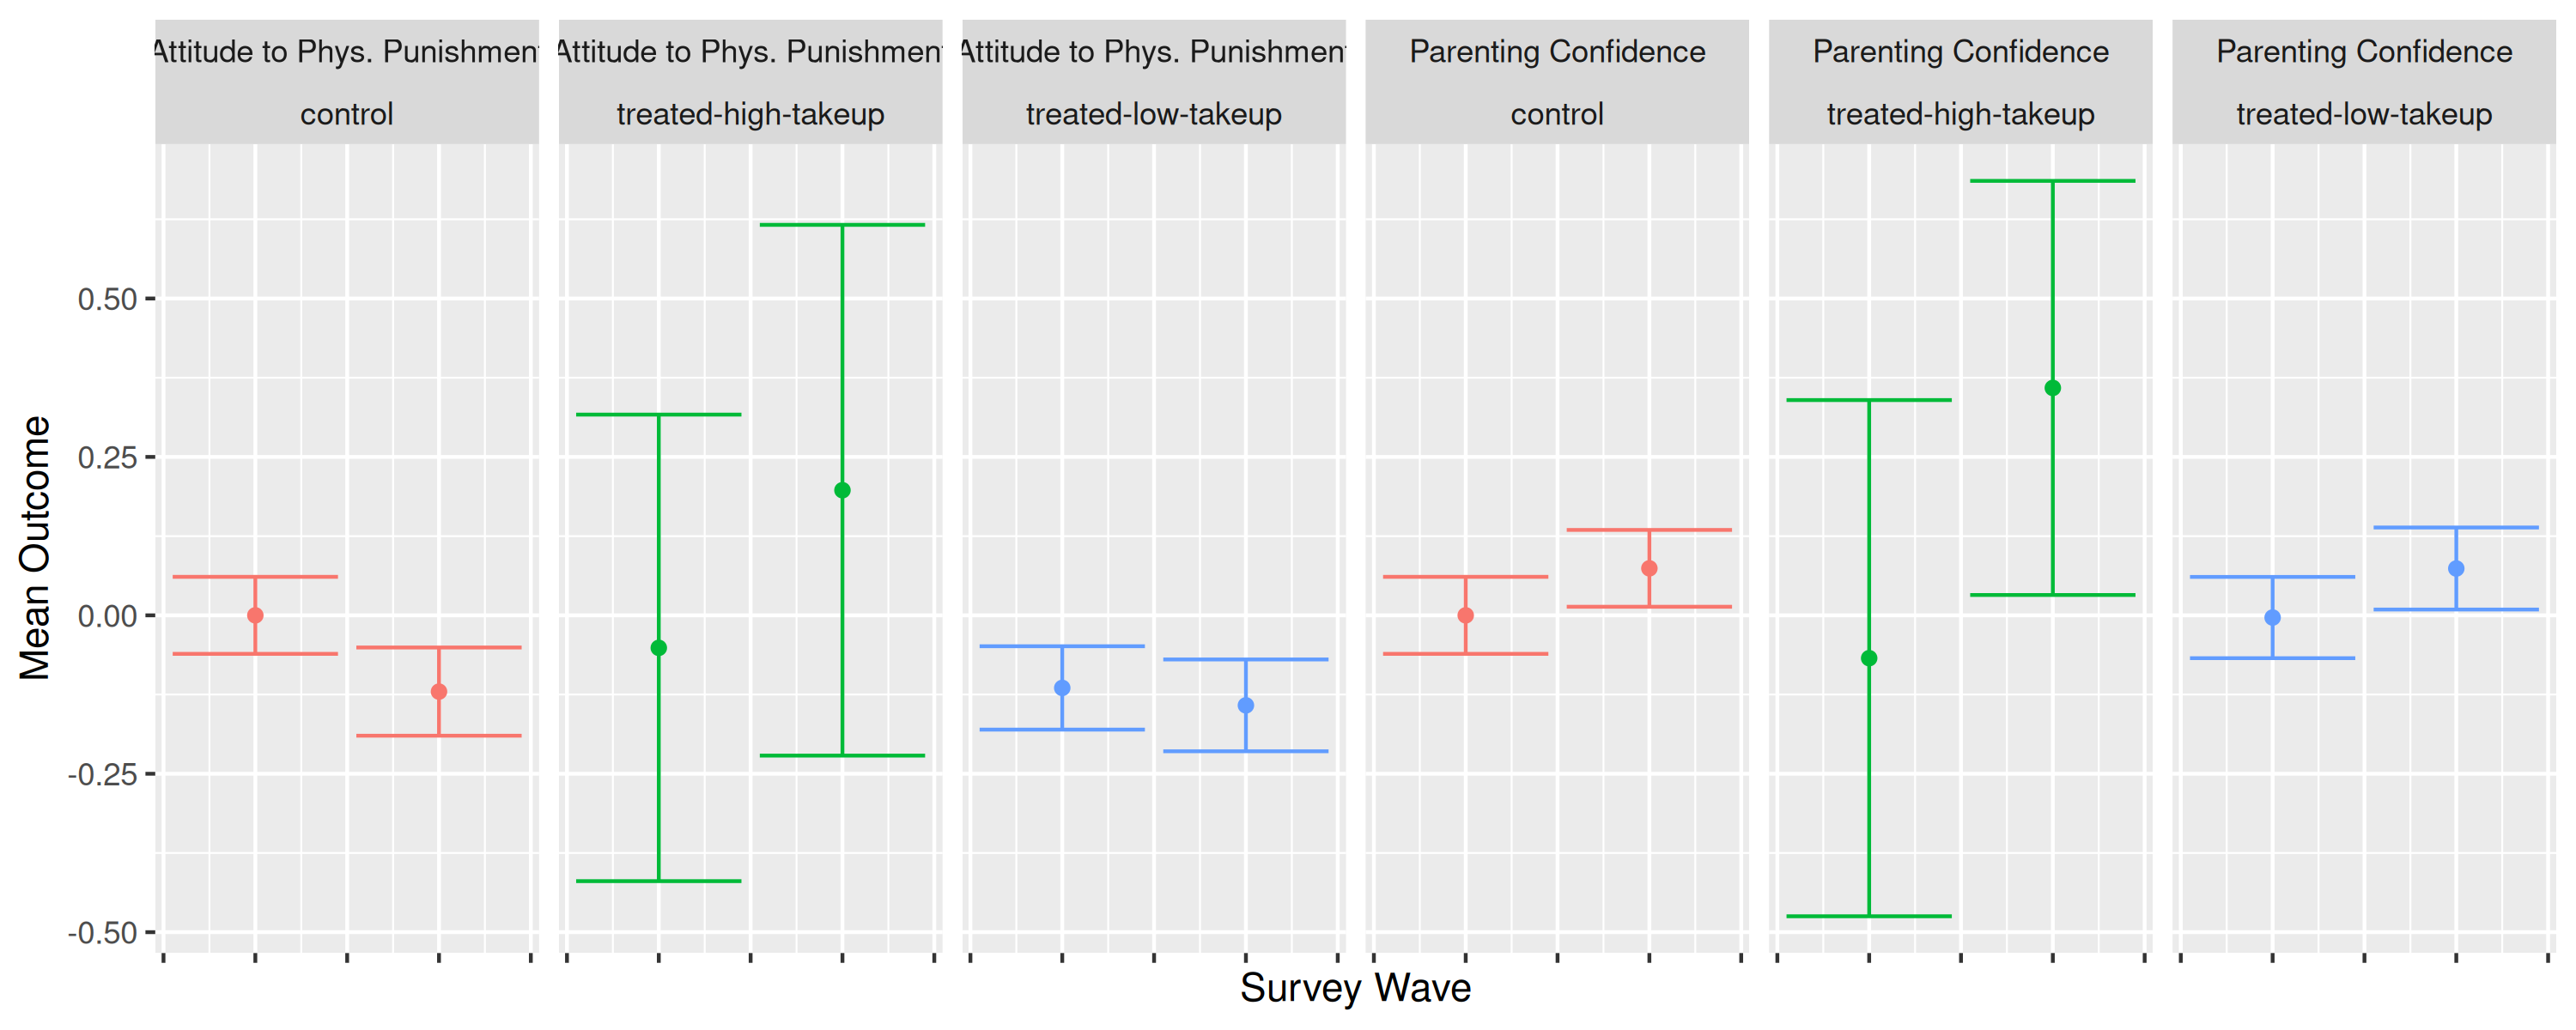
\includegraphics[width=\textwidth]{chapters/03-bebbo/plots/pre_post/Pooled: Parenting Confidence.png}
\caption{Confidence and Attitudes}
\label{fig:confidence-and-attitudes-pre-post}
\end{figure}


\subsection{Practices}

These four constructs all relate to practices and behaviors of the parent. No significant effect was found for any of the behaviors. There is some evidence of selective take-up in the group that scores worse on parenting practices, both in the raw data but also in the takeup regressions. The raw regression results suggest that Activities Past 24h show suggestive evidence of impact, but the raw data shows that the much of the improvement is driven by those in the treated group who did not take-up the treatment, which gives credence to the assumption that this could be statistical noise and is why we have corrected for multiple testing.

\input{chapters/03-bebbo/regressions/Pooled: OLS - Endline - Practices.tex}

\begin{figure}[H]
  \centering
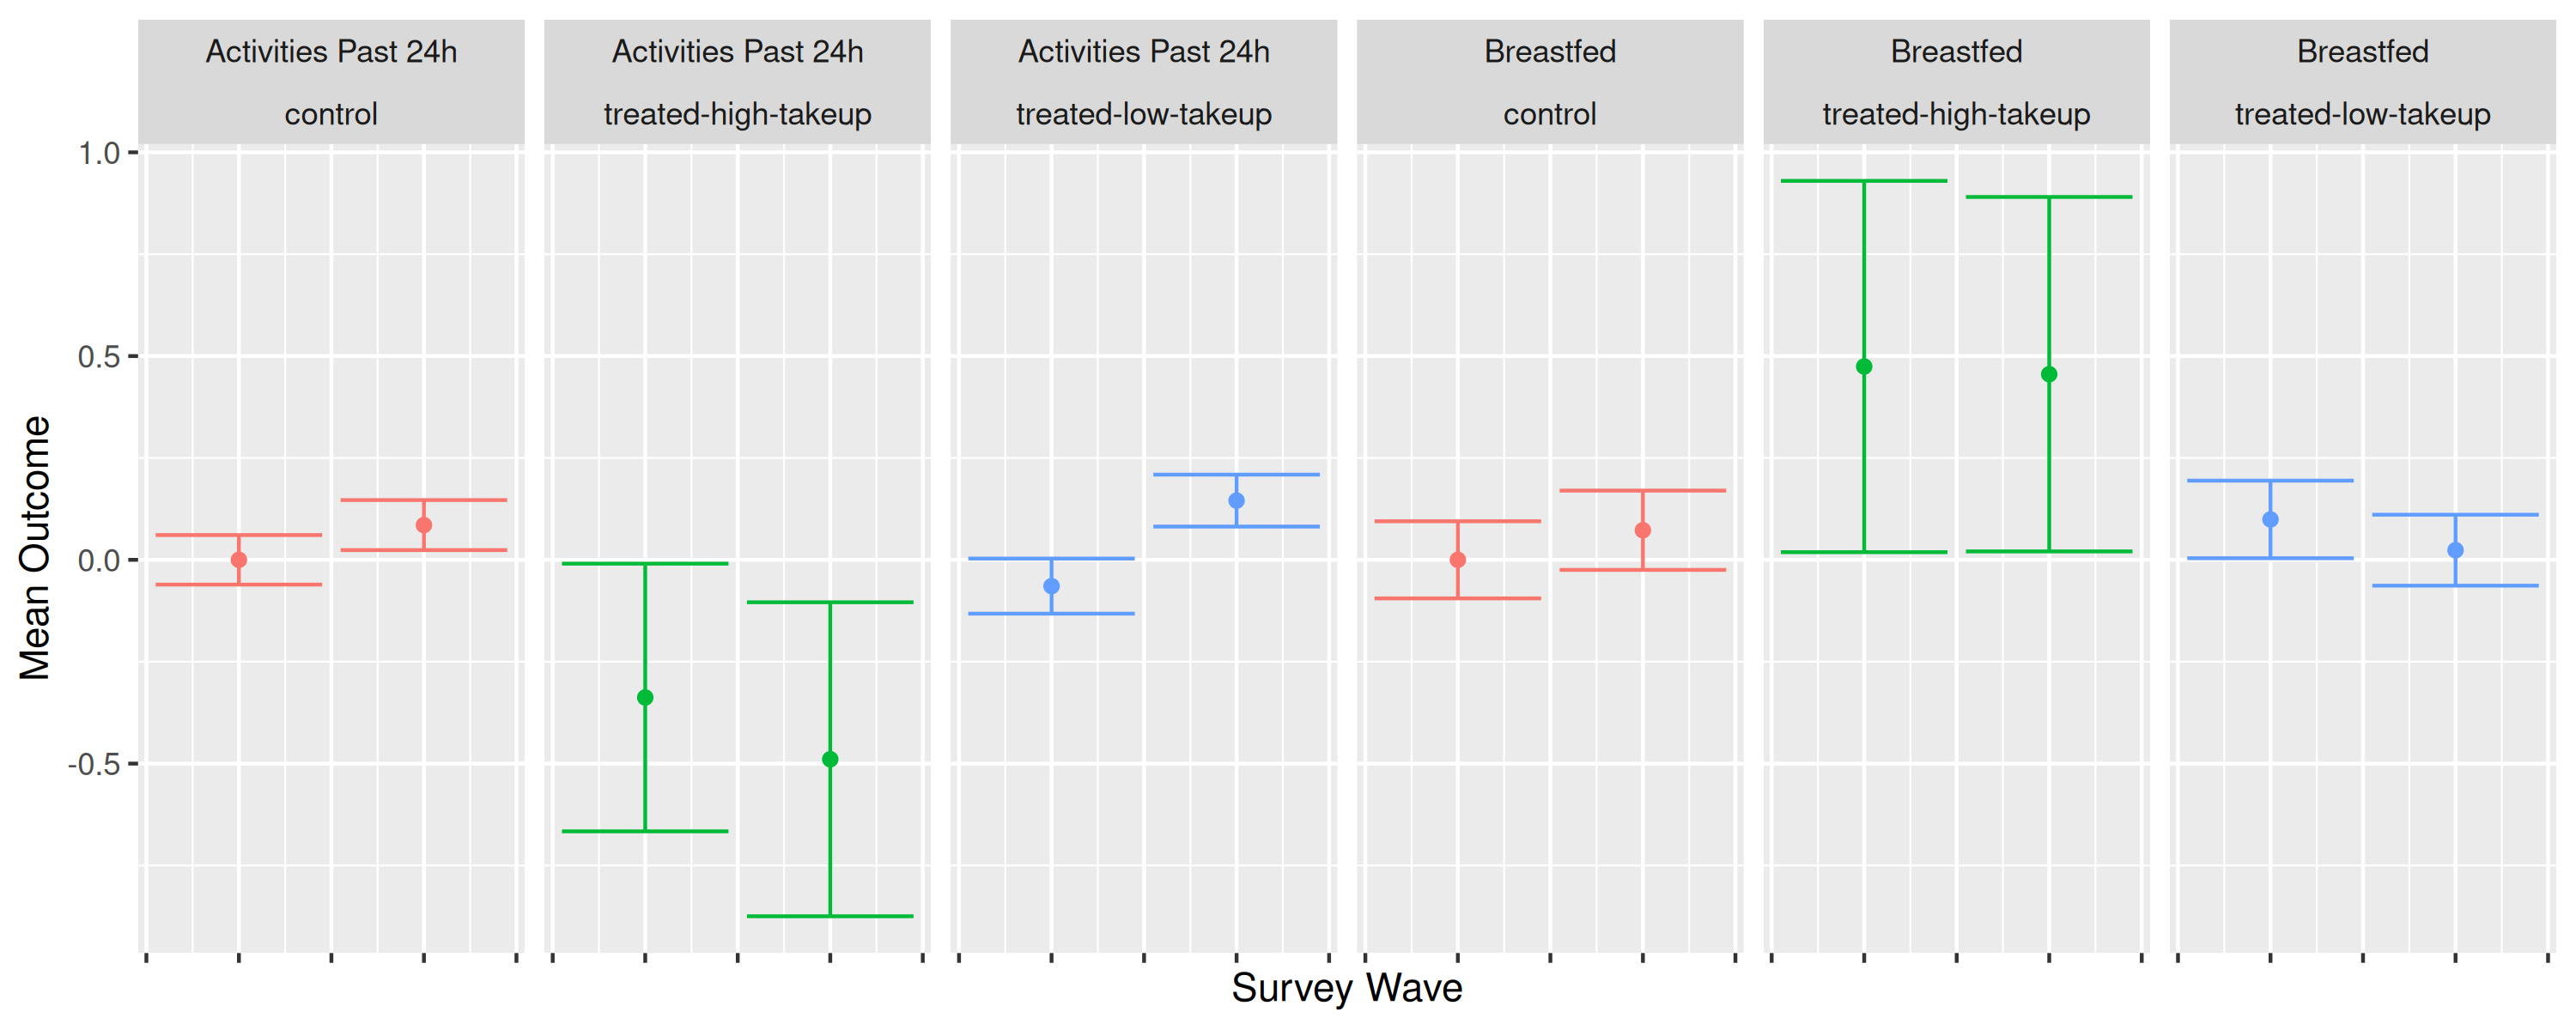
\includegraphics[width=0.9\textwidth]{chapters/03-bebbo/plots/pre_post/Pooled: Breastfed.png}
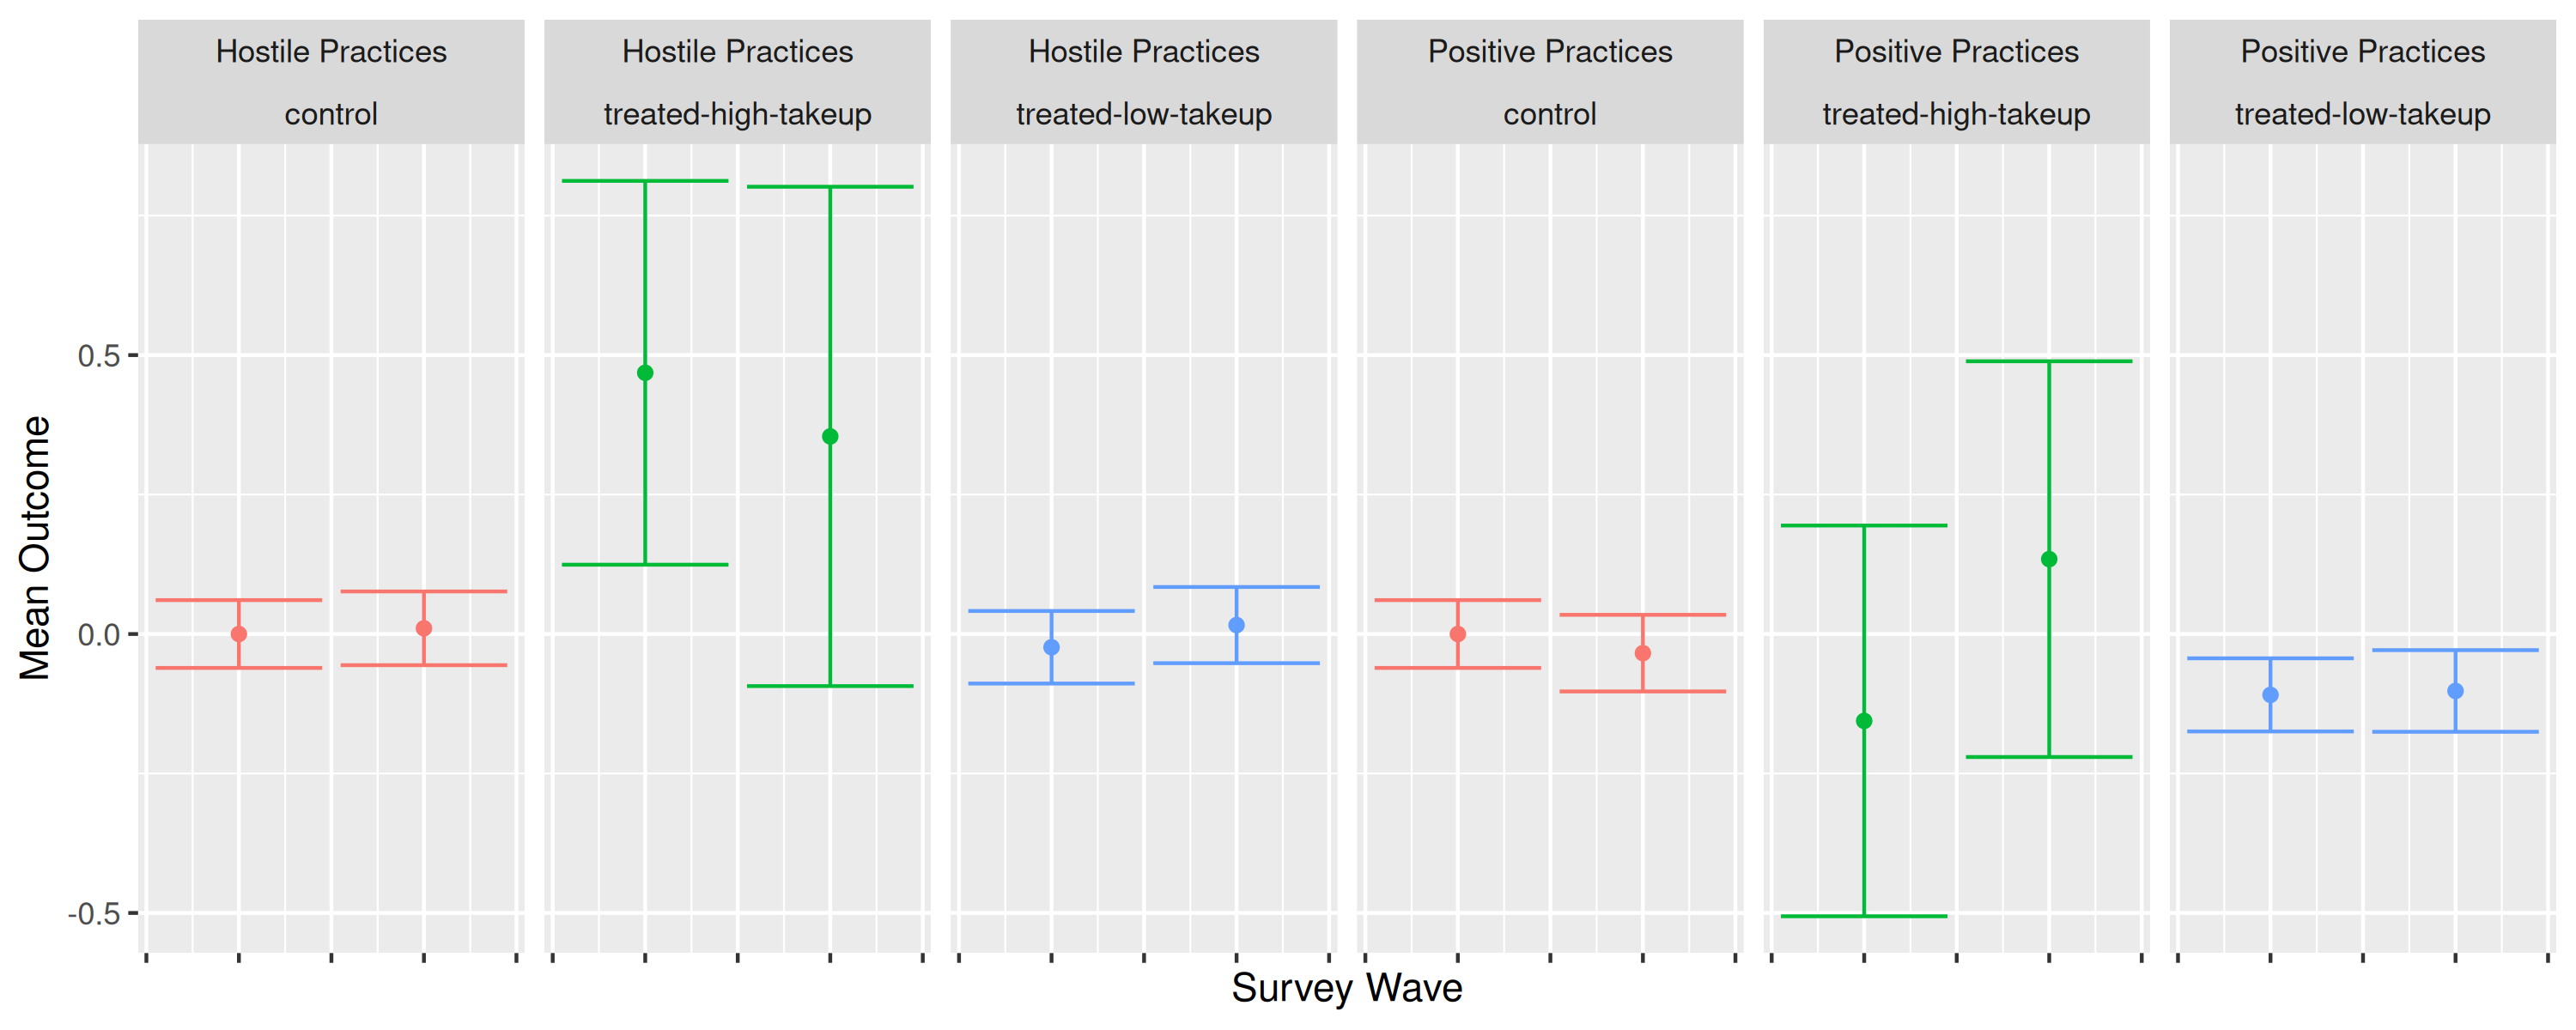
\includegraphics[width=0.9\textwidth]{chapters/03-bebbo/plots/pre_post/Pooled: Positive Practices.png}
\caption{Practices}
\label{fig:practices-pre-post}
\end{figure}


\subsection{Limitations}

We list below some methodological limitations of the study that should be taken into consideration when interpreting the current study results:

\begin{enumerate}
\item Our study population consists of volunteers recruited via social media ads. Participants in voluntary studies or surveys may be different in significant ways to the general population and those differences may limit the external validity of these findings. Findings related to app usage can, and have been, validated with app usage data from the general population of app downloaders. All other findings related to survey results, however, have not been validated
\item The majority of respondents scored well on the baseline assessment and thus it is likely that they could not improve much in the endline due to this ceiling effect. While this might be due to a failure in the creation of the survey instrument, it could also be an example in the bias of the sample population (i.e., they are all better-than-average caregivers). Note that, as discussed in the next section, this can also indicate a need to better target Bebbo to respective audiences and contexts.
\item Due to the online nature of the study, we could only use a short survey. This limited us to use further established scales to measure other related outcomes (e.g., other positive or negative parenting practices).
\item Due to the online nature of the study, the attrition rates were high. However, our analyses indicated no evidence of selective attrition across the treatment arms. Furthermore, the high attrition rates did not lead to a statistical power problem, such that the study had sufficient sample size to detect any effects, if they existed.
\end{enumerate}


\subsection{Conclusions and Recommendations}

The analysis conducted on the effects of promoting (i.e., the intent-to-treat analyses) or using (i.e. treatment effect on the treated analyses) the Bebbo app on caregivers with children aged 0-6 did not reveal any statistically significant impact on key outcomes of interest.

One of the main contributing factors to this outcome appears to be the low engagement levels of the users with the Bebbo app. Despite the potential benefits of mobile apps in fostering continuous engagement, data indicate that a significant proportion of users, both within our study and in general (as shown by the app monitoring data), tend to abandon the app after a short period. Specifically, 76\% of users in our study who complied with the suggestion to download Bebbo abandoned it after the first day. This is also in line with app usage data outside of our study, which shows that over 86\% of users abandon it after one day.

For an app to influence behaviors and attitudes, it must be attractive and engaging enough to retain a large portion of the target audience over time. While take-up defined as “had at least one learning event” was 29.9\% in our study, which would be enough to measure impacts, it’s reasonable to believe that in order to have an impact on these outcomes, especially behaviors and attitudes, participants would need to use the app continuously.

If we consider the advantage of an app over a static website or informational flyer, the advantage comes through continued usage (it is available on your home screen, can send you push notifications, etc.). Given that only 3\% used the app more than three days, we would not expect to see much of an impact of this app on this population. Furthermore, despite our attempts to predict app usage from baseline characteristics, the study did not yield significant predictions; while there was a trend suggesting that parents less likely to engage in activities with their children were more inclined to use the parenting app.

That being said, there were other factors that might have contributed to the lack of discovery of an impact that are in-and-of-themselves interesting. In particular:

\begin{enumerate}
\item There seemed to be a priming effect of the baseline survey, especially for questions related to knowledge, such as “when is your child’s next vaccination due.” This could imply that a prompt itself can change parent’s knowledge and raises questions on how best to position Bebbo to leverage this possibility.
\item The majority of respondents scored well on the baseline assessment. If the respondents were representative of the general population, this would imply that most caregivers in these countries are already knowledgeable and following many good practices.
\end{enumerate}

In conclusion, while the promotion of the Bebbo app did not result in significant effects on the target population, the study provides valuable insights into the challenges of promoting and sustaining engagement with mobile apps for parenting. Future app-based interventions should consider strategies to enhance user engagement and retention to maximize the potential impact. In particular, for an intervention to have an impact on a population level, it is not sufficient to engage a small percentage of the population intensely. One needs to engage a large percentage of the population. This is in contrast to the majority of private-sector apps, who only need a small portion of the population to engage in order to make a successful business.

This is also highlights an important weakness of apps themselves, as population-level interventions. Apps by their nature create upfront friction (download and install), which is rewarded with long-term, deeper engagement. The priming effect we see in this study, where asking questions at baseline improves knowledge at endline regardless of intervention or takeup, implies that informational campaigns to promote awareness might have a significant impact---at significantly greater scale than hiding that information inside an app.

Finally, taken another way, these results might also imply that it is difficult to create a ``generic, all-purpose parenting app'' that improves multiple elements of parenting. The general high-level of scores among most parents could imply that interventions need to focus on targeting those who are struggling the most, not the general population.




\numberwithin{table}{section}
\numberwithin{figure}{section}


\section{Additional Plots}

\begin{figure}[H]
\begin{minipage}{.5\textwidth}
    \centering
    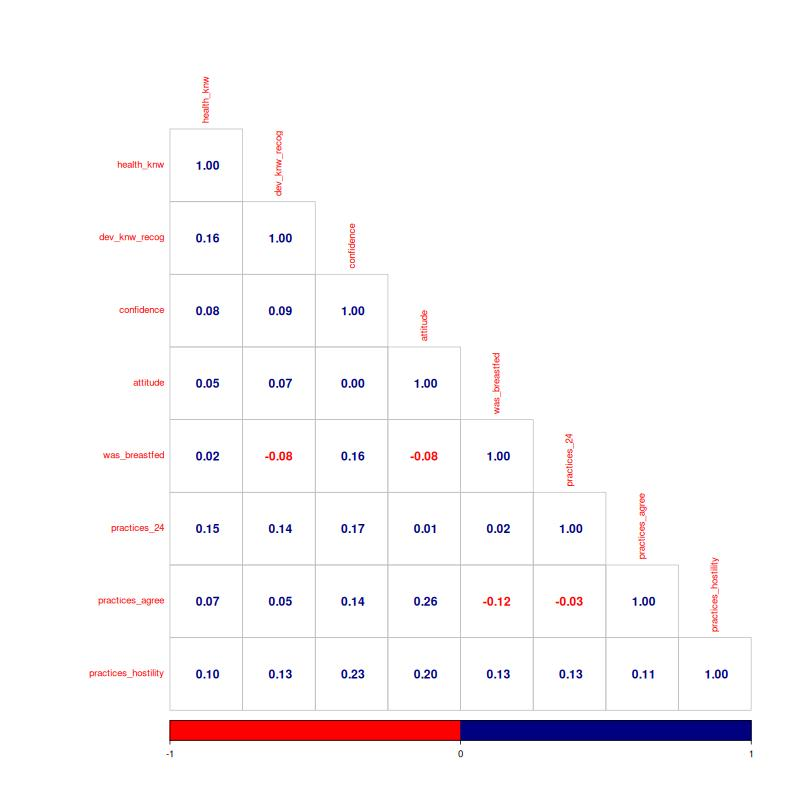
\includegraphics[scale=0.33]{chapters/03-bebbo/descriptives/plots/correlations_constructs_Serbia_Baseline.jpg}
    \caption{Construct Correlations - Serbia}
    \label{fig:serbia correlations}
\end{minipage}%
\begin{minipage}{.5\textwidth}
    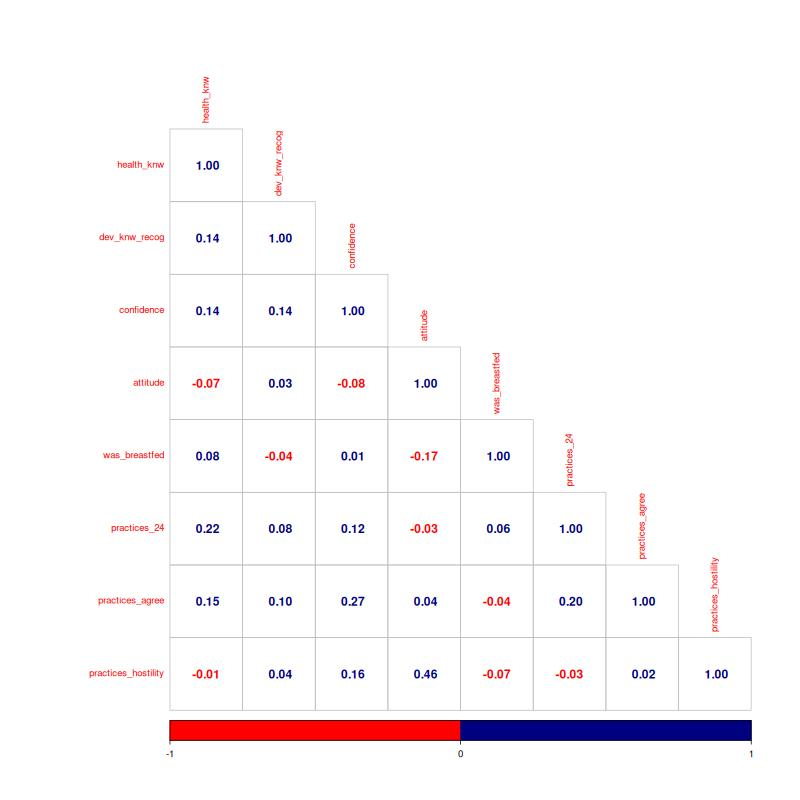
\includegraphics[scale=0.33]{chapters/03-bebbo/descriptives/plots/correlations_constructs_Bulgaria_Baseline.jpg}
    \caption{Construct Correlations - Bulgaria}
    \label{fig:bulgaria correlations}
\end{minipage}%
\end{figure}

\begin{figure}[H]
  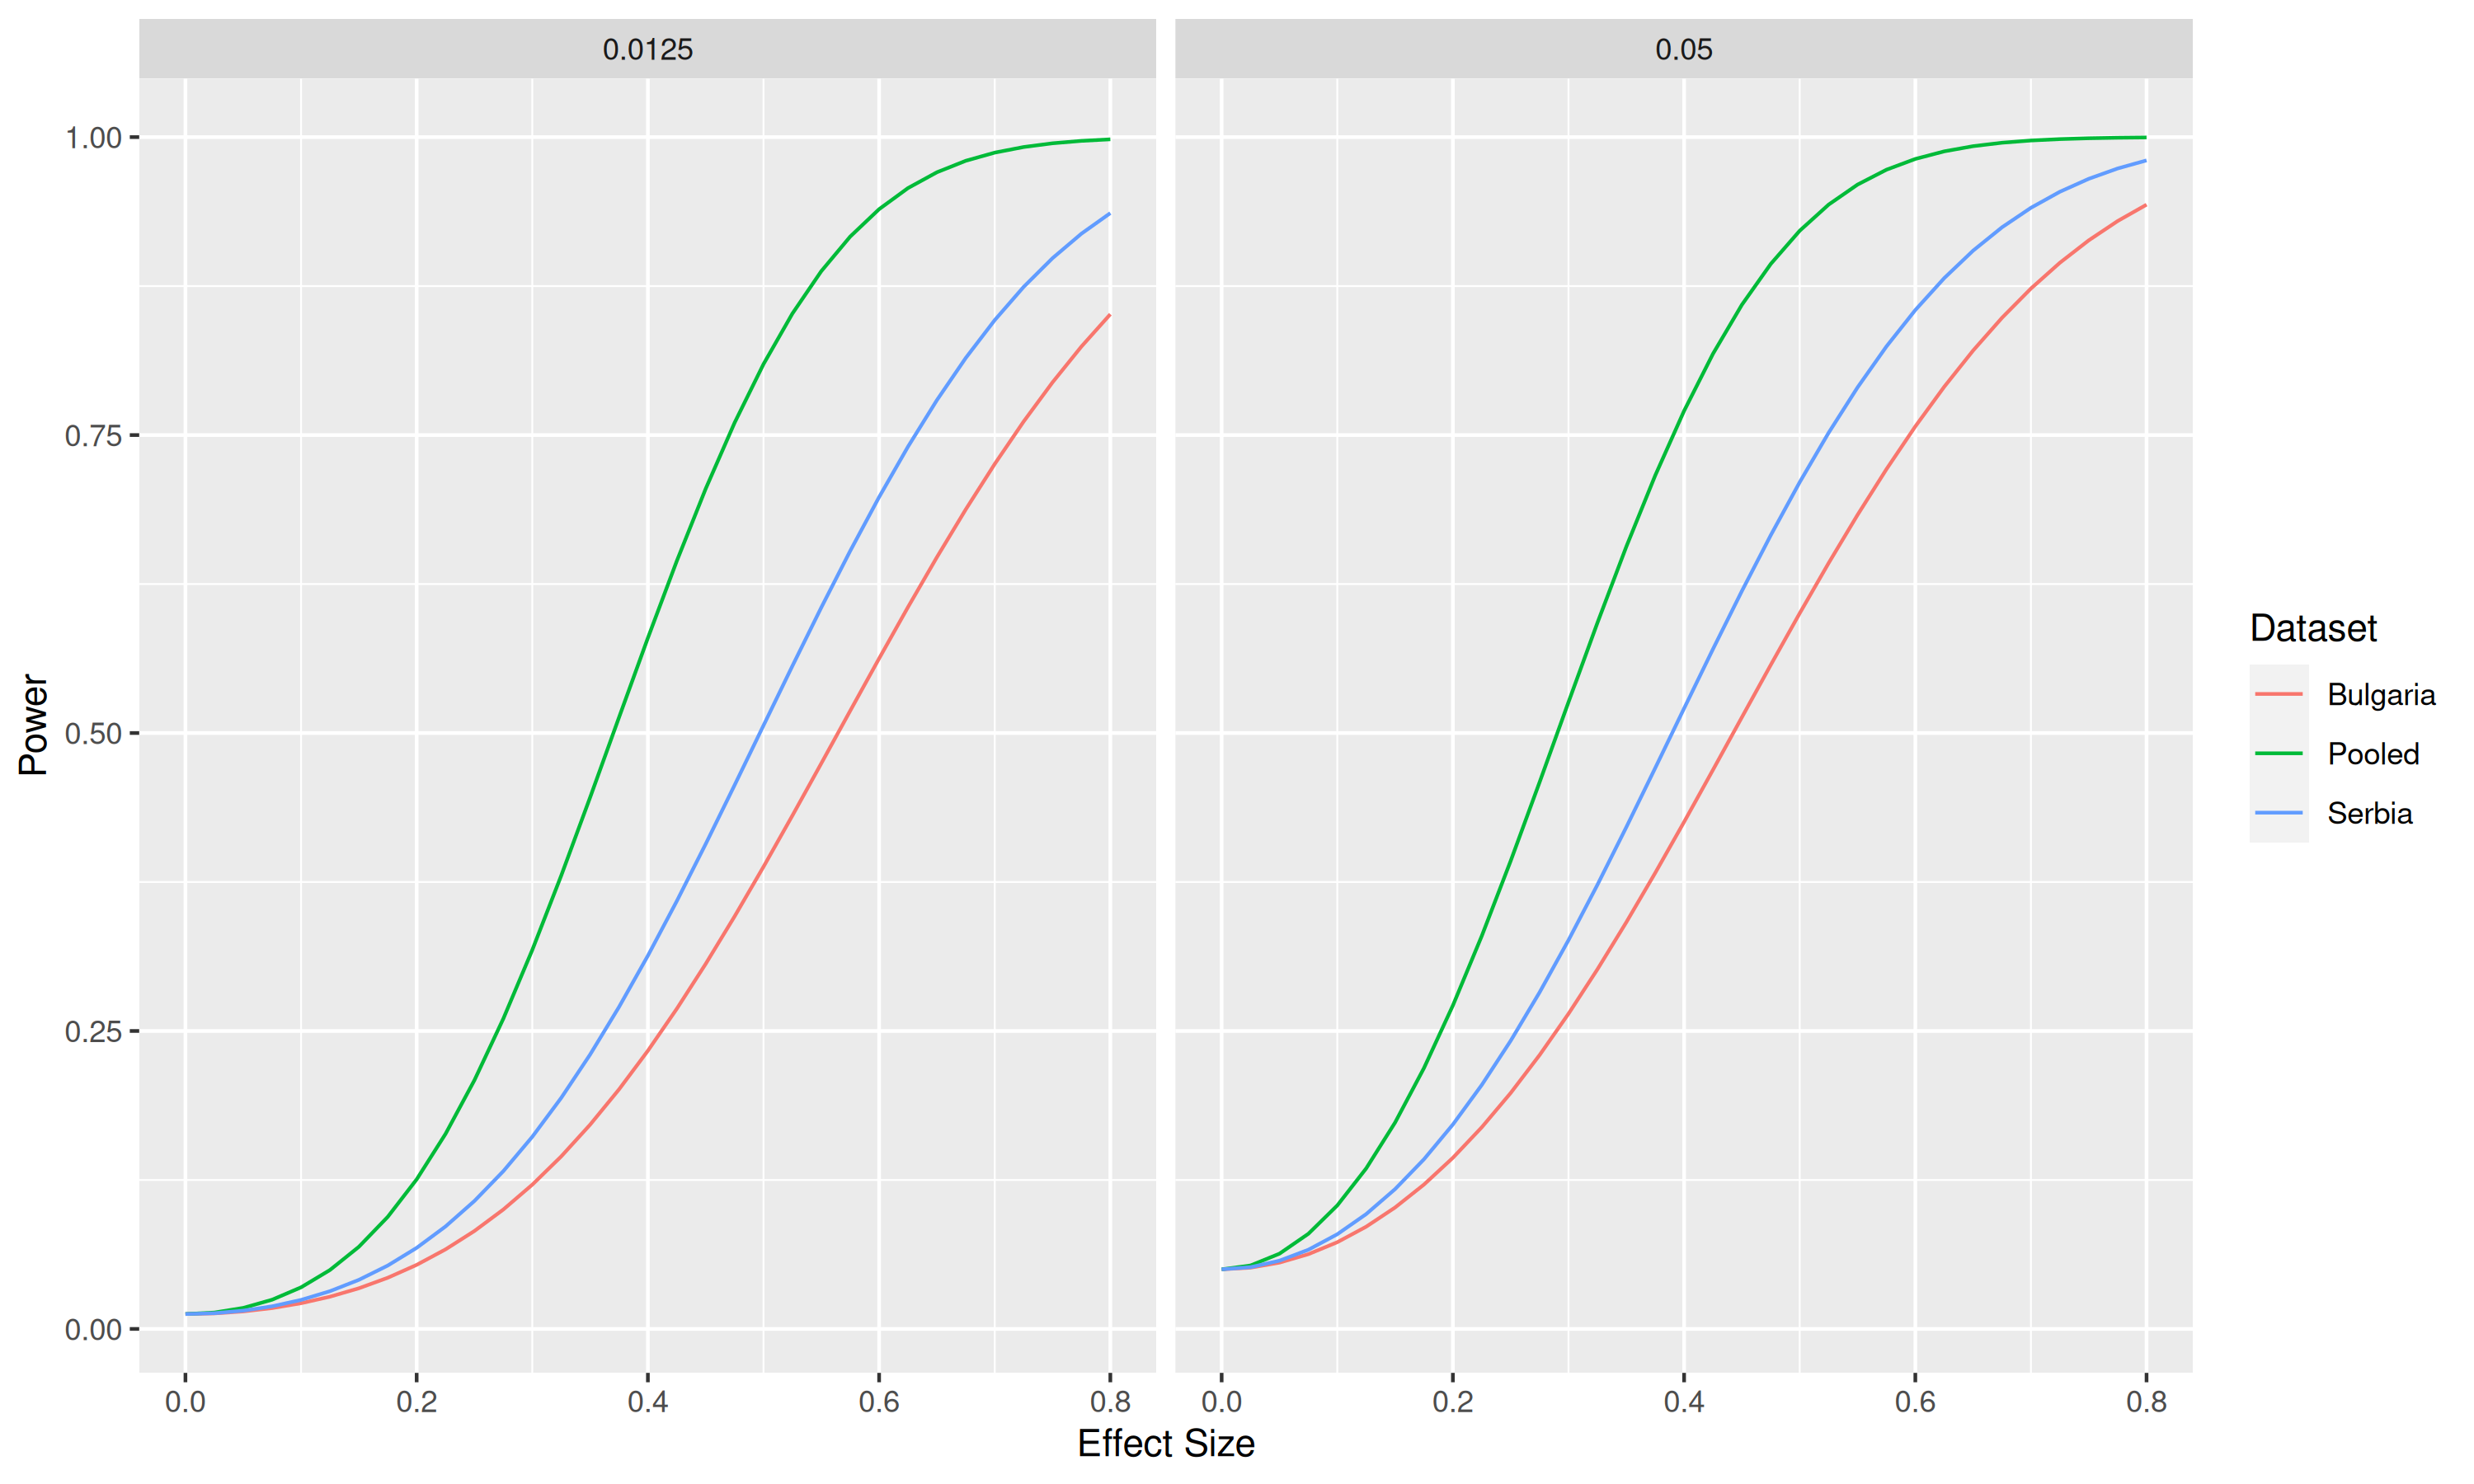
\includegraphics[width=1.0\textwidth]{chapters/03-bebbo/plots/Power Calculations.png}
  \caption{Power Analysis at 28\% Takeup}
  \label{fig:Power Analysis}
\end{figure}

\clearpage


\begin{figure}[H]
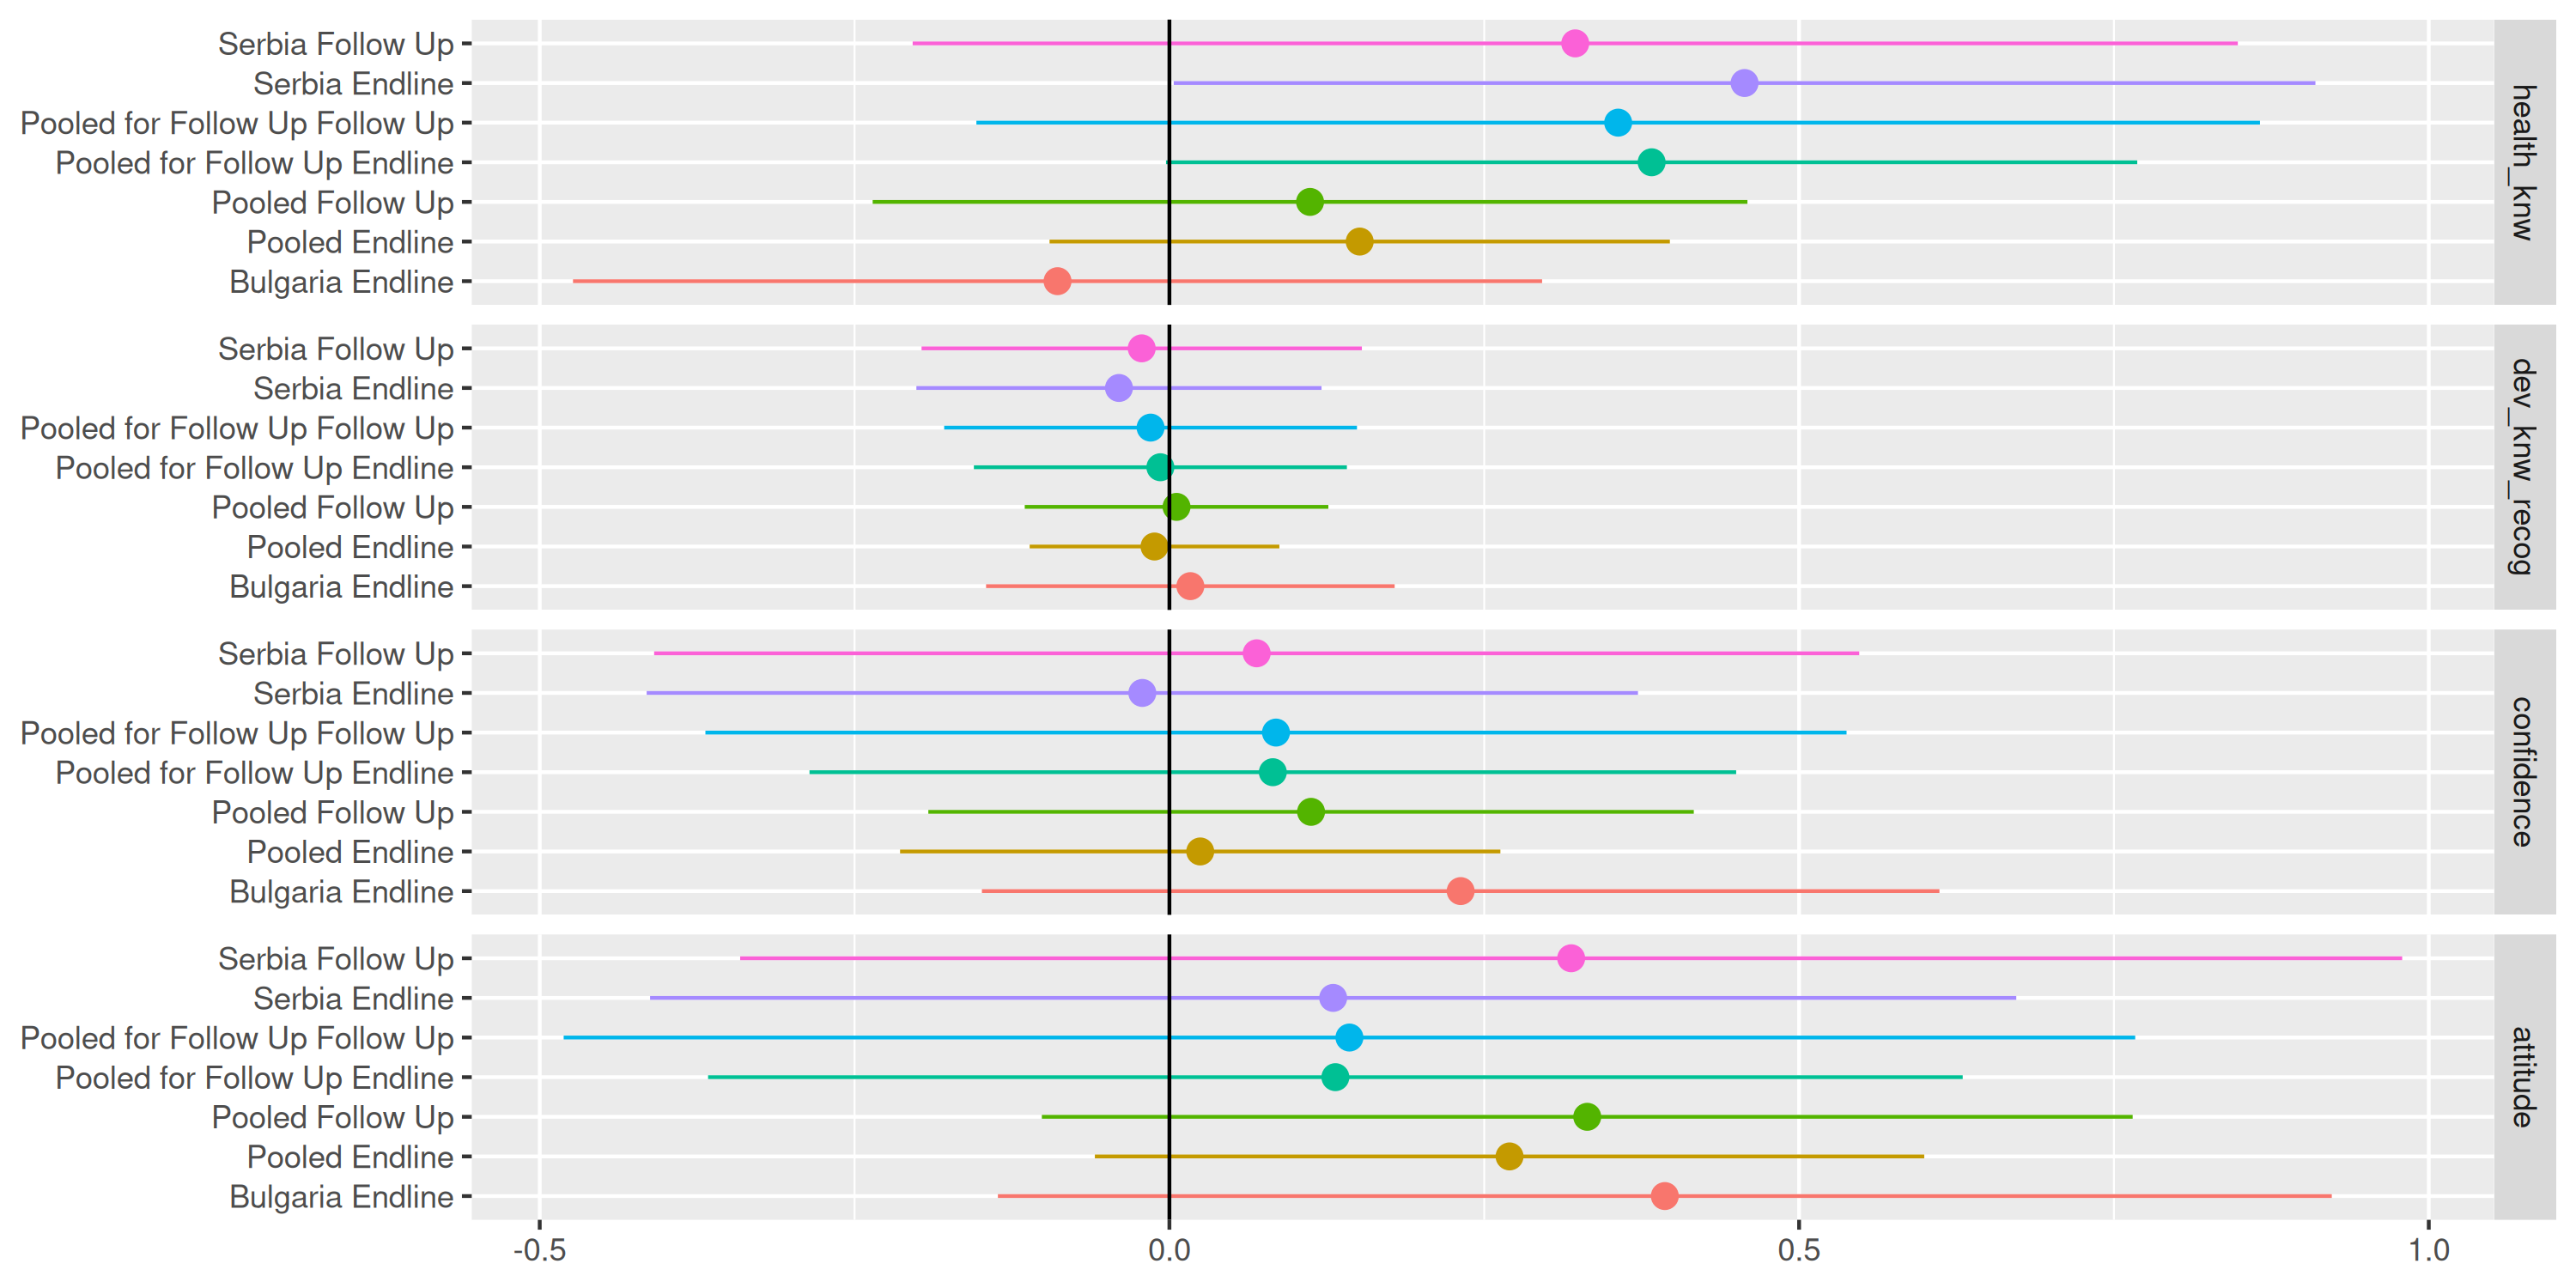
\includegraphics[width=\textwidth]{chapters/03-bebbo/plots/Adjusted Coefficient Plot Knowledge and Attitudes.png}
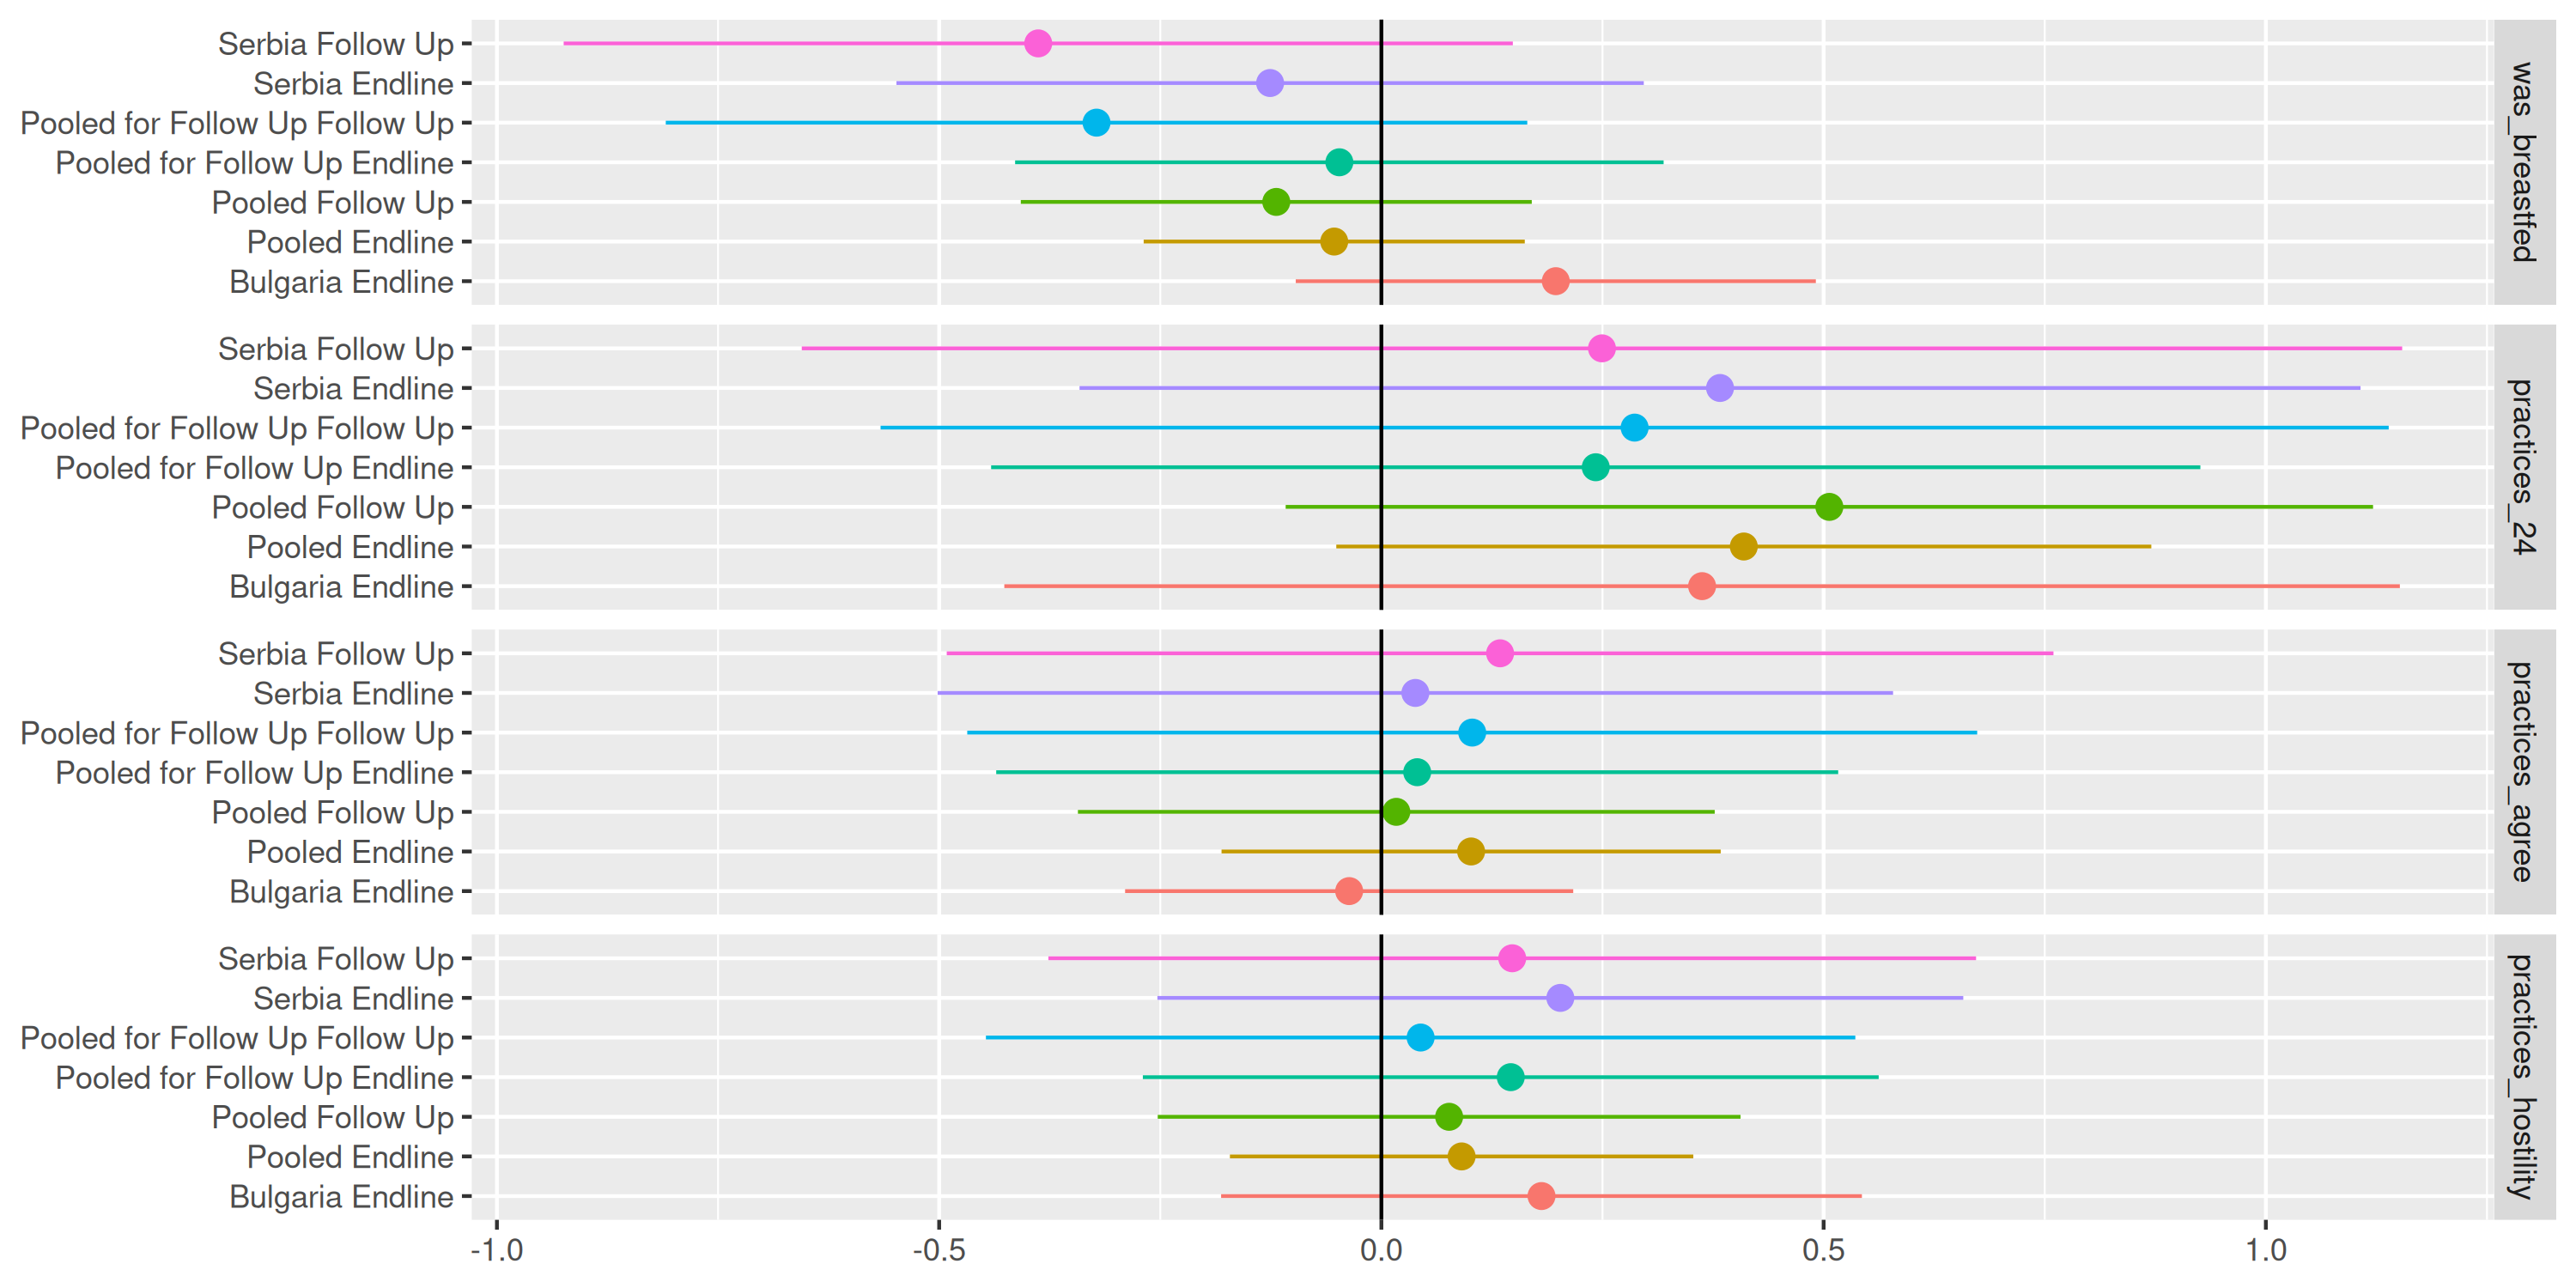
\includegraphics[width=\textwidth]{chapters/03-bebbo/plots/Adjusted Coefficient Plot Practices.png}
\caption{Adjusted Coefficient Plots of 2SLS in Pooled Dataset}
\end{figure}

\section{Per Country Descriptives and Attrition Rates}


\input{chapters/03-bebbo/descriptives/tables/Outcome Construct Descriptives Serbia Baseline}
\input{chapters/03-bebbo/descriptives/tables/Outcome Construct Descriptives Bulgaria Baseline}

\input{chapters/03-bebbo/descriptives/tables/Attrition: Serbia.tex}
\input{chapters/03-bebbo/descriptives/tables/Attrition: Bulgaria.tex}

\section{Subgroup Regressions}

While the study was not designed for subgroup analysis and thus they are very subject to false positives from multiple testing, it is instructive to run some subgroup regressions.

In particular, we run the regression on the subset that failed the vaccine knowledge question in the first wave (for children aged 0-2).

\input{chapters/03-bebbo/regressions/Vaccine Failures Subgroup OLS - Endline.tex}

For illustrative purposes, we also present results for families that have a 0-2 years old child. No impact is found for this group.

\input{chapters/03-bebbo/regressions/Only Children 0-2: OLS - Endline - Knowledge and Awareness.tex}
\input{chapters/03-bebbo/regressions/Only Children 0-2: OLS - Endline - Confidence and Attitudes.tex}
\input{chapters/03-bebbo/regressions/Only Children 0-2: OLS - Endline - Practices.tex}

\section{ToT Regressions}

Given that there is no significant impact measured in our evaluation regressions, we do not estimate the impact to be anything other than zero. That being said, the point estimates might still be suggestive evidence and one effective way to measure the point estimates of the impact is through an analysis of the treatment effect on the treated (ToT).

We estimate this using an instrumental variable model given the monotonicity assumption of treatment (\cite{Imbens2015}), which assumes that people are not less likely to download and use the Bebbo app in the treatment group. To estimate our instrumental variable model, we use 2-stage least squares:
\begin{align*}
y_{i} - y^{b}_i &= \gamma_1 + \beta \hat{z}_{i} + \gamma_2X_{i} + \epsilon_i \\
z_{i} &= \gamma_3 + \gamma_4 T_{i} + \gamma_5X_{i} + \delta_i
\end{align*}

Where $z_i$ is a binary indicator of takeup based on the recorded app-usage data and $\hat{z_i}$ the predicted takeup based on the first stage regression. Once again, parameter of interest is $\beta$.


\input{chapters/03-bebbo/regressions/Pooled: 2SLS - Endline - Knowledge and Awareness.tex}

\input{chapters/03-bebbo/regressions/Pooled: 2SLS - Endline - Confidence and Attitudes.tex}

\input{chapters/03-bebbo/regressions/Pooled: 2SLS - Endline - Practices.tex}

\section{Country Specific Regressions}

For robustness checks, we run regressions on the individual countries.

\input{chapters/03-bebbo/regressions/Serbia: OLS - Endline - Practices.tex}
\input{chapters/03-bebbo/regressions/Serbia: OLS - Endline - Knowledge and Awareness.tex}
\input{chapters/03-bebbo/regressions/Serbia: OLS - Endline - Confidence and Attitudes.tex}

\input{chapters/03-bebbo/regressions/Bulgaria: OLS - Endline - Knowledge and Awareness.tex}
\input{chapters/03-bebbo/regressions/Bulgaria: OLS - Endline - Confidence and Attitudes.tex}
\input{chapters/03-bebbo/regressions/Bulgaria: OLS - Endline - Practices.tex}

% \input{chapters/03-bebbo/regressions/Serbia: 2SLS - Endline - Knowledge and Awareness.tex}
% \input{chapters/03-bebbo/regressions/Serbia: 2SLS - Endline - Confidence and Attitudes.tex}
% \input{chapters/03-bebbo/regressions/Serbia: 2SLS - Endline - Practices.tex}

% \input{chapters/03-bebbo/regressions/Bulgaria: 2SLS - Endline - Knowledge and Awareness.tex}
% \input{chapters/03-bebbo/regressions/Bulgaria: 2SLS - Endline - Confidence and Attitudes.tex}
% \input{chapters/03-bebbo/regressions/Bulgaria: 2SLS - Endline - Practices.tex}

\section{Follow-up Regressions}

As discussed in the text, due to low usage and high attrition, we restricted our primary analysis to the endline survey. That being said, we provide the regressions for the follow-up survey as well in this section.

\input{chapters/03-bebbo/regressions/Pooled for Follow Up: OLS - Follow Up - Knowledge and Awareness.tex}
\input{chapters/03-bebbo/regressions/Pooled for Follow Up: OLS - Follow Up - Confidence and Attitudes.tex}
\input{chapters/03-bebbo/regressions/Pooled for Follow Up: OLS - Follow Up - Practices.tex}

% \input{chapters/03-bebbo/regressions/Pooled for Follow Up: 2SLS - Follow Up - Knowledge and Awareness.tex}
% \input{chapters/03-bebbo/regressions/Pooled for Follow Up: 2SLS - Follow Up - Confidence and Attitudes.tex}
% \input{chapters/03-bebbo/regressions/Pooled for Follow Up: 2SLS - Follow Up - Practices.tex}

% \input{chapters/03-bebbo/regressions/Serbia: OLS - Follow Up - Knowledge and Awareness.tex}
% \input{chapters/03-bebbo/regressions/Serbia: OLS - Follow Up - Confidence and Attitudes.tex}
% \input{chapters/03-bebbo/regressions/Serbia: OLS - Follow Up - Practices.tex}

% \input{chapters/03-bebbo/regressions/Serbia: 2SLS - Follow Up - Knowledge and Awareness.tex}
% \input{chapters/03-bebbo/regressions/Serbia: 2SLS - Follow Up - Confidence and Attitudes.tex}
% \input{chapters/03-bebbo/regressions/Serbia: 2SLS - Follow Up - Practices.tex}

% \input{chapters/03-bebbo/regressions/Bulgaria: OLS - Follow Up - Knowledge and Awareness.tex}
% \input{chapters/03-bebbo/regressions/Bulgaria: OLS - Follow Up - Confidence and Attitudes.tex}
% \input{chapters/03-bebbo/regressions/Bulgaria: OLS - Follow Up - Practices.tex}

% \input{chapters/03-bebbo/regressions/Bulgaria: 2SLS - Follow Up - Knowledge and Awareness.tex}
% \input{chapters/03-bebbo/regressions/Bulgaria: 2SLS - Follow Up - Confidence and Attitudes.tex}
% \input{chapters/03-bebbo/regressions/Bulgaria: 2SLS - Follow Up - Practices.tex}

